\chapter{Parallel Computing}\label{parallel}

\section{Overview}\label{parallel:overview}

This chapter describes the various parallel computing capabilities
provided by Dakota.  We begin with a high-level summary.

Dakota has been designed to exploit a wide range of parallel
computing resources such as those found in a desktop multiprocessor
workstation, a network of workstations, or a massively parallel
computing platform. This parallel computing capability is a critical
technology for rendering real-world engineering design problems
computationally tractable. Dakota employs the concept of
\emph{multilevel parallelism}, which takes simultaneous advantage of
opportunities for parallel execution from multiple sources:

\textbf{Parallel Simulation Codes}: Dakota works equally well with both
serial and parallel simulation codes.

\textbf{Concurrent Execution of Analyses within a Function Evaluation}:
Some engineering design applications call for the use of multiple
simulation code executions (different disciplinary codes, the same
code for different load cases or environments, etc.) in order to
evaluate a single response data set\footnote{the term ``function 
evaluation'' is used broadly to mean any individual data request 
from an iterative algorithm} (e.g., objective functions and
constraints) for a single set of parameters. If these simulation code
executions are independent (or if coupling is enforced at a higher
level), Dakota can perform them concurrently.

\textbf{Concurrent Execution of Function Evaluations within an Iterator}: 
With very few exceptions, the iterative algorithms described in
Chapters~\ref{ps}--\ref{nls} all provide opportunities
for the concurrent evaluation of response data sets for different
parameter sets. Whenever there exists a set of function evaluations
that are independent, Dakota can perform them in parallel.

\textbf{Concurrent Execution of Sub-Iterators within a Meta-iterator
  or Nested Model}: The advanced methods described in
Chapter~\ref{adv_meth} are examples of meta-iterators, and the
advanced model recursions described in
Sections~\ref{adv_models:mixed_uq}--\ref{adv_models:ouu} all utilize
nested models. Both of these cases generate sets of iterator
subproblems that can be executed concurrently. For example, the
Pareto-set and multi-start strategies generate sets of optimization
subproblems. Similarly, optimization under uncertainty
(\ref{adv_models:ouu}) generates sets of uncertainty quantification
subproblems. Whenever these subproblems are independent, Dakota can
perform them in parallel.

It is important to recognize that these four parallelism sources can
be combined recursively.  For example, a meta-iterator can schedule
and manage concurrent iterators, each of which may manage concurrent
function evaluations, each of which may manage concurrent analyses,
each of which may execute on multiple processors.  Moreover, more than
one source of sub-iteration concurrency can be exploited when
combining meta-iteration and nested model sources.  In an extreme
example, defining the Pareto frontier for mixed-integer nonlinear
programming under mixed aleatory-epistemic uncertainty might exploit
up to four levels of nested sub-iterator concurrency in addition to
available levels from function evaluation concurrency, analysis
concurrency, and simulation parallelism.  The majority of application
scenarios, however, will employ one to two levels of parallelism.

Navigating the body of this chapter: The range of capabilities is
extensive and can be daunting at first; therefore, this chapter takes
an incremental approach in first describing the simplest single-level
parallel computing models (Section~\ref{parallel:SLP}) using
asynchronous local, message passing, and hybrid approaches.  More
advanced uses of Dakota can build on this foundation to exploit
multiple levels of parallelism, as described in
Section~\ref{parallel:MLP}.

The chapter concludes with a discussion of using Dakota with
applications that run as independent MPI processes (parallel
application tiling, for example on a large compute cluster).  This
last section is a good quick start for interfacing Dakota to your
parallel (or serial) application on a cluster.


% In the following sections, the parallel algorithms available in this
% Dakota release are listed followed by descriptions of the software
% components that enable parallelism, approaches for utilizing these
% components, and input specification and execution details for
% running parallel Dakota studies.

\subsection{Categorization of parallelism}\label{parallel:overview:cat}

To understand the parallel computing possibilities, it is instructive
to first categorize the opportunities for exploiting parallelism into
four main areas~\cite{Eld98a}, consisting of coarse-grained and
fine-grained parallelism opportunities within algorithms and their
function evaluations:

\begin{enumerate}
\item \emph{Algorithmic coarse-grained parallelism}: This parallelism
  involves the concurrent execution of independent function
  evaluations, where a ``function evaluation'' is defined as a data
  request from an algorithm (which may involve value, gradient, and
  Hessian data from multiple objective and constraint functions). This
  concept can also be extended to the concurrent execution of multiple
  ``iterators'' within a ``meta-iterator.'' Examples of algorithms
  containing coarse-grained parallelism include:
  \begin{itemize}
  \item \emph{Gradient-based algorithms}: finite difference gradient
    evaluations, speculative optimization, parallel line search.

  \item \emph{Nongradient-based algorithms}: genetic algorithms (GAs),
    pattern search (PS), Monte Carlo sampling.

  \item \emph{Approximate methods}: design of computer experiments for
    building surrogate models.

  \item \emph{Concurrent sub-iteration}: optimization under
    uncertainty, branch and bound, multi-start local search, Pareto
    set optimization, island-model GAs.
  \end{itemize}

\item \emph{Algorithmic fine-grained parallelism}: This involves
  computing the basic computational steps of an optimization algorithm
  (i.e., the internal linear algebra) in parallel. This is primarily
  of interest in large-scale optimization problems and simultaneous
  analysis and design (SAND).

\item \emph{Function evaluation coarse-grained parallelism}: This
  involves concurrent computation of separable parts of a single
  function evaluation. This parallelism can be exploited when the
  evaluation of the response data set requires multiple independent
  simulations (e.g. multiple loading cases or operational
  environments) or multiple dependent analyses where the coupling is
  applied at the optimizer level (e.g., multiple disciplines in the
  individual discipline feasible formulation~\cite{Den94a}).

\item \emph{Function evaluation fine-grained parallelism}: This
  involves parallelization of the solution steps within a single
  analysis code.  Support for massively parallel simulation continues
  to grow in areas of nonlinear mechanics, structural dynamics, heat
  transfer, computational fluid dynamics, shock physics, and many
  others.
\end{enumerate}

By definition, coarse-grained parallelism requires very little
inter-processor communication and is therefore ``embarrassingly
parallel,'' meaning that there is little loss in parallel efficiency
due to communication as the number of processors increases. However,
it is often the case that there are not enough separable computations
on each algorithm cycle to utilize the thousands of processors
available on massively parallel machines. For example, a thermal safety
application~\cite{Eld96a} demonstrated this limitation with a pattern
search optimization in which the maximum speedup exploiting
\emph{only} coarse-grained algorithmic parallelism was shown to be
limited by the size of the design problem (coordinate pattern search
has at most $2n$ independent evaluations per cycle for $n$ design
variables).

Fine-grained parallelism, on the other hand, involves much more
communication among processors and care must be taken to avoid the
case of inefficient machine utilization in which the communication
demands among processors outstrip the amount of actual computational
work to be performed. For example, a chemically-reacting flow
application~\cite{Eld98a} illustrated this limitation for a simulation
of fixed size in which it was shown that, while simulation run time
did monotonically decrease with increasing number of processors, the
relative parallel efficiency $\hat{E}$ of the computation for fixed
model size decreased rapidly (from $\hat{E} \approx 0.8$ at 64
processors to $\hat{E} \approx 0.4$ at 512 processors). This was due
to the fact that the total amount of computation was approximately
fixed, whereas the communication demands were increasing rapidly with
increasing numbers of processors. Therefore, there is a practical
limit on the number of processors that can be employed for
fine-grained parallel simulation of a particular model size, and only
for extreme model sizes can thousands of processors be efficiently
utilized in studies exploiting fine-grained parallelism alone.

These limitations point us to the exploitation of multiple levels of
parallelism, in particular the combination of coarse-grained and
fine-grained approaches. This will allow us to execute fine-grained
parallel simulations on sets of processors where they are most
efficient and then replicate this efficiency with many coarse-grained
instances involving one or more levels of nested job scheduling.  
%From a software perspective, coarse-grained parallelism by
%itself (many instances of a single-processor simulation) and
%fine-grained parallelism by itself (a single instance of a large
%multiprocessor simulation) can be considered to cover two ends of a
%spectrum, and we are interested in also supporting anywhere in between
%(any number of instances of any size simulation).  Single-level
%parallelism approaches (the extremes of this spectrum) are described
%in Section~\ref{parallel:SLP}, and multilevel parallelism approaches
%(middle of the spectrum) are discussed in Section~\ref{parallel:MLP}.

%The available concurrency in function evaluation parallelism is
%determined by the aspects of a particular systems analysis
%application, and is therefore highly application-dependent.
%Algorithmic parallelism, on the other hand, is largely determined by
%the selection and configuration of a particular algorithm.  These
%selection possibilities within Dakota are outlined in the following
%section.


\subsection{Parallel Dakota algorithms} \label{parallel:algorithms}

In Dakota, the following parallel algorithms, comprised of iterators
and meta-iterators, provide support for coarse-grained algorithmic
parallelism.  Note that, even if a particular algorithm is serial in
terms of its data request concurrency, other concurrency sources
(e.g., function evaluation coarse-grained and fine-grained
parallelism) may still be available.

\subsubsection{Parallel iterators}\label{parallel:algorithms:iterators}

\begin{itemize}
\item Gradient-based optimizers: CONMIN, DOT, NLPQL, NPSOL, and OPT++
  can all exploit parallelism through the use of Dakota's native finite
  differencing routine (selected with \texttt{method\_source dakota}
  in the responses specification), which will perform concurrent
  evaluations for each of the parameter offsets. For \texttt{n}
  variables, forward differences result in an $n+1$ concurrency and
  central differences result in a $2n+1$ concurrency. In addition,
  CONMIN, DOT, and OPT++ can use speculative gradient
  techniques~\cite{Byr88} to obtain better parallel load balancing. By
  speculating that the gradient information associated with a given
  line search point will be used later and computing the gradient
  information in parallel at the same time as the function values, the
  concurrency during the gradient evaluation and line search phases
  can be balanced. NPSOL does not use speculative gradients since this
  approach is superseded by NPSOL's gradient-based line search in
  user-supplied derivative mode.  NLPQL also supports a distributed
  line search capability for generating concurrency~\cite{Sch04}.
  Finally, finite-difference Newton algorithms can exploit additional
  concurrency in numerically evaluating Hessian matrices. % TO DO: which?

\item Nongradient-based optimizers: HOPSPACK, JEGA methods, and most
  SCOLIB methods support parallelism.  HOPSPACK and SCOLIB methods
  exploit parallelism through the use of Dakota's concurrent function
  evaluations; however, there are some limitations on the levels of
  concurrency and asynchrony that can be exploited.  These are detailed
  in the Dakota Reference Manual. Serial SCOLIB methods include
  Solis-Wets (\texttt{coliny\_solis\_wets}) and certain
  \texttt{exploratory\_moves} options (\texttt{adaptive\_pattern} and
  \texttt{multi\_step}) in pattern search
  (\texttt{coliny\_pattern\_search}).  OPT++ PDS (\texttt{optpp\_pds})
  and NCSU DIRECT (\texttt{ncsu\_direct}) are also currently serial
  due to incompatibilities in Dakota and OPT++/NCSU parallelism
  models.  Finally, \texttt{coliny\_pattern\_search} and
  \texttt{asynch\_pattern\_search} support dynamic job queues managed
  with nonblocking synchronization.

\item Least squares methods: in an identical manner to the
  gradient-based optimizers, NL2SOL, NLSSOL, and Gauss-Newton can
  exploit parallelism through the use of Dakota's native finite
  differencing routine. In addition, NL2SOL and Gauss-Newton can use
  speculative gradient techniques to obtain better parallel load
  balancing. NLSSOL does not use speculative gradients since this
  approach is superseded by NLSSOL's gradient-based line search in
  user-supplied derivative mode.

\item Surrogate-based minimizers: \texttt{surrogate\_based\_local},
  \texttt{surrogate\_based\_global}, and \texttt{efficient\_global}
  all support parallelism in the initial surrogate construction, but
  subsequent concurrency varies.  In the case of
  \texttt{efficient\_global}, only a single point is generated for
  evaluation for each subsequent cycle and there is no derivatove
  concurrency for this point.  In the case of
  \texttt{surrogate\_based\_local}, only a single point is generated
  per subsequent cycle, but derivative concurrency for numerical
  gradient or Hessian evaluations may be available.  And in the case
  of \texttt{surrogate\_based\_global}, multiple points may be
  generated on each subsequent cycle, depending on the multipoint
  return capability of specific minimizers.

\item Parameter studies: all parameter study methods (\texttt{vector},
  \texttt{list}, \texttt{centered}, and \texttt{multidim}) support
  parallelism. These methods avoid internal synchronization points, so
  all evaluations are available for concurrent execution.

\item Design of experiments: all \texttt{dace} (\texttt{grid},
  \texttt{random}, \texttt{oas}, \texttt{lhs}, \texttt{oa\_lhs},
  \texttt{box\_behnken}, and \texttt{central\_composite}),
  \texttt{fsu\_quasi\_mc} (\texttt{halton} and \texttt{hammersley}),
  \texttt{fsu\_cvt}, and \texttt{psuade\_moat} methods support
  parallelism.

\item Uncertainty quantification: all nondeterministic methods
  (sampling, reliability, stochastic expansion, and epistemic) support
  parallelism. In the case of gradient-based methods (local
  reliability, local interval estimation), parallelism can be exploited
  through the use of Dakota's native finite differencing routine for
  computing gradients.  In the case of many global methods (e.g.,
  global reliability, global interval estimation, polynomial chaos),
  initial surrogate construction is highly parallel, but any subsequent
  (adaptive) refinement may have greater concurrency restrictions
  (including a single point per refinement cycle in some cases).
\end{itemize}

\subsubsection{Advanced methods}\label{parallel:algorithms:adv_meth}

Certain advanced methods support concurrency in multiple iterator
executions. Currently, the methods which can exploit this level of
parallelism are:

\begin{itemize}
\item Hybrid minimization: when the sequential hybrid transfers multiple
solution points between methods, single-point minimizers will be executed
concurrently using each of the transferred solution points.

%\item Branch and bound: optimization meta-iterator for mixed-integer
%nonlinear programming with noncategorical discrete variables.

\item Pareto-set optimization: a meta-iterator for multiobjective
  optimization using the simple weighted-sum approach for computing
  sets of points on the Pareto front of nondominated solutions.

\item Multi-start iteration: a meta-iterator for executing multiple
  instances of an iterator from different starting points.
\end{itemize}

%In the branch and bound case, the available iterator concurrency grows
%as the tree develops more branches, so some of the iterator servers
%may be idle in the initial phases. Similarly, 
The hybrid minimization case will display varying levels of iterator 
concurrency based on differing support of multipoint solution input/output 
between iterators; however, the use of multiple parallel configurations 
among the iterator sequence should prevent parallel inefficiencies.  On 
the other hand, pareto-set and multi-start have a fixed set of jobs to 
perform and should exhibit good load balancing.

\subsubsection{Parallel models}\label{parallel:algorithms:models}

Parallelism support in model classes (see Chapter~\ref{models}) is an
important issue for 
%variable scaling (see Section~\ref{opt:additional:scaling}) and 
advanced model recursions such as surrogate-based minimization,
optimization under uncertainty, and mixed aleatory-epistemic UQ (see
Chapters~\ref{adv_meth} and~\ref{adv_models}).  Support is as follows:

\begin{itemize}
\item Single model: parallelism is managed as specified in the model's
  associated \texttt{interface} instance.

\item Recast model: most parallelism is forwarded on to the sub-model.
  An exception to this is finite differencing in the presence of
  variable scaling.  Since it is desirable to perform offsets in the
  scaled space (and avoid minimum step size tolerances), this
  parallelism is not forwarded to the sub-model, instead being enacted
  at the recast level.

\item Data fit surrogate model: parallelism is supported in the
  construction of global surrogate models via the concurrent
  evaluation of points generated by design of experiments methods.
  Local and multipoint approximations evaluate only a single point at
  a time, so concurrency is available only from any numerical
  differencing required for gradient and Hessian data.  Since the
  top-level iterator is interfaced only with the (inexpensive)
  surrogate, no parallelism is exploited there.  Load balancing can be
  an important issue when performing evaluations to (adaptively)
  update existing surrogate models.

\item Hierarchical surrogate model: parallelism is supported for the
  low or the high fidelity models, and in some contexts, for both
  models at the same time.  In the multifidelity optimization context,
  the optimizer is interfaced only with the low-fidelity model, and
  the high-fidelity model is used only for verifications and
  correction updating.  For this case, the algorithmic coarse-grained
  parallelism supported by the optimizer is enacted on the low
  fidelity model and the only parallelism available for high fidelity
  executions arises from any numerical differencing required for
  high-fidelity gradient and Hessian data.  In contexts that compute
  model discrepancies, such as multifidelity UQ, the algorithmic
  concurrency involves evaluation of both low and high fidelity
  models, so parallel schedulers can exploit simultaneous concurrency
  for both models.

\item Nested model: concurrent executions of the optional interface
  and concurrent executions of the sub-iterator are supported and are
  synchronized in succession.  Currently, synchronization is blocking
  (all concurrent evaluations are completed before new batches are
  scheduled); nonblocking schedulers (see~\ref{parallel:SLP}) may be
  supported in time.  Nested model concurrency and meta-iterator
  concurrency (Section~\ref{parallel:algorithms:adv_meth}) may be
  combined within an arbitrary number of levels of recursion.  Primary
  clients for this capability include optimization under uncertainty
  and mixed aleatory-epistemic UQ (see Section~\ref{models:nested}).
\end{itemize}


\section{Single-level parallelism} \label{parallel:SLP}


Dakota's parallel facilities support a broad range of computing
hardware, from custom massively parallel supercomputers on the high
end, to clusters and networks of workstations in the middle range, to
desktop multiprocessors on the low end. Given the reduced scale in the
middle to low ranges, it is more common to exploit only one of the
levels of parallelism; however, this can still be quite effective in
reducing the time to obtain a solution.  Three single-level
parallelism models will be discussed, and are depicted in
Figure~\ref{parallel:figure03}:

\begin{figure}[ht]
  \centering
  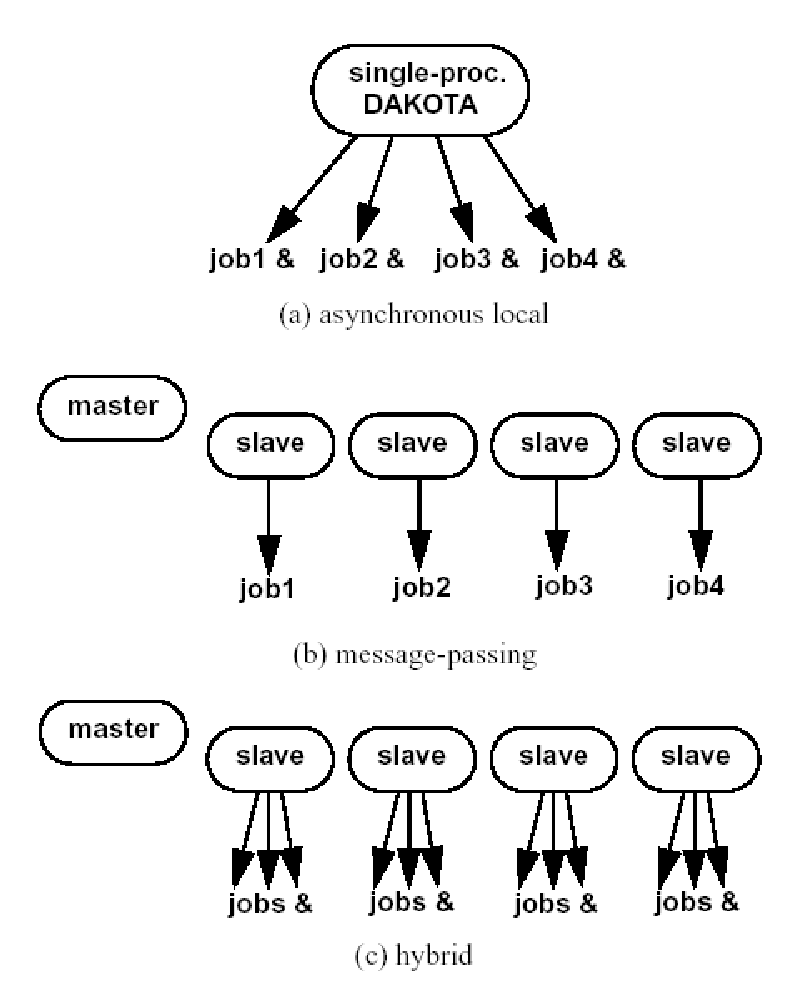
\includegraphics[width=60mm]{images/ex_in_hy_job_management}
  \caption{External, internal, and hybrid job management.}
  \label{parallel:figure03}
\end{figure}

\begin{itemize}
\item \emph{asynchronous local}: Dakota executes on a single processor,
but launches multiple jobs concurrently using asynchronous job launching
techniques.

\item \emph{message passing}: Dakota executes in parallel using message
passing to communicate between processors.  A single job is launched
per processor using synchronous job launching techniques.

\item \emph{hybrid}: a combination of message passing and asynchronous
local.  Dakota executes in parallel across multiple processors and
launches concurrent jobs on each processor.
\end{itemize}

In each of these cases, jobs are executing concurrently and must be
collected in some manner for return to an algorithm.  Blocking and
nonblocking approaches are provided for this, where the blocking
approach is used in most cases:
\begin{itemize}
\item \emph{blocking synchronization}: all jobs in the queue are
completed before exiting the scheduler and returning the set of
results to the algorithm.  The job queue fills and then empties
completely, which provides a synchronization point for the algorithm.

\item \emph{nonblocking synchronization}: the job queue is dynamic,
with jobs entering and leaving continuously.  There are no defined
synchronization points for the algorithm, which requires specialized
algorithm logic (only currently supported by
\texttt{coliny\_pattern\_search} and \texttt{asynch\_pattern\_search}, which
are sometimes referred to as ``fully asynchronous'' algorithms).
\end{itemize}

Given these job management capabilities, it is worth noting that the
popular term ``asynchronous'' can be ambiguous when used in isolation.
In particular, it can be important to qualify whether one is referring
to ``asynchronous job launch'' (synonymous with any of the three
concurrent job launch approaches described above) or ``asynchronous
job recovery'' (synonymous with the latter nonblocking job
synchronization approach).


%\subsection{Local Simulation Invocation Components}\label{parallel:SLP:local}
\subsection{Asynchronous Local Parallelism}\label{parallel:SLP:local}

This section describes software components which manage simulation
invocations local to a processor. These invocations may be either
synchronous (i.e., blocking) or asynchronous (i.e., nonblocking).
Synchronous evaluations proceed one at a time with the evaluation
running to completion before control is returned to Dakota.
Asynchronous evaluations are initiated such that control is returned
to Dakota immediately, prior to evaluation completion, thereby
allowing the initiation of additional evaluations which will execute
concurrently.

The synchronous local invocation capabilities are used in two
contexts: (1) by themselves to provide serial execution on a single
processor, and (2) in combination with Dakota's message-passing
schedulers to provide function evaluations local to each
processor. Similarly, the asynchronous local invocation capabilities
are used in two contexts: (1) by themselves to launch concurrent jobs
from a single processor that rely on external means (e.g., operating
system, job queues) for assignment to other processors, and (2) in
combination with Dakota's message-passing schedulers to provide a
hybrid parallelism (see Section~\ref{parallel:SLP:hybrid}).  Thus,
Dakota supports any of the four combinations of synchronous or
asynchronous local combined with message passing or without.

Asynchronous local schedulers may be used for managing concurrent
function evaluations requested by an iterator or for managing
concurrent analyses within each function evaluation.  The former
iterator/evaluation concurrency supports either blocking (all jobs in
the queue must be completed by the scheduler) or nonblocking (dynamic
job queue may shrink or expand) synchronization, where blocking
synchronization is used by most iterators and nonblocking
synchronization is used by fully asynchronous algorithms such as
\texttt{asynch\_pattern\_search} and \texttt{coliny\_pattern\_search}.  The
latter evaluation/analysis concurrency is restricted to blocking
synchronization.  The ``Asynchronous Local'' column in
Table~\ref{parallel:table01} summarizes these capabilities.

Dakota supports three local simulation invocation approaches based on
the direct function, system call, and fork simulation interfaces.  For
each of these cases, an input filter, one or more analysis drivers,
and an output filter make up the interface, as described in
Section~\ref{interfaces:components}.

\subsubsection{Direct function synchronization}\label{parallel:SLP:local:direct}

The direct function capability may be used synchronously. Synchronous
operation of the direct function simulation interface involves a
standard procedure call to the input filter, if present, followed by
calls to one or more simulations, followed by a call to the output
filter, if present (refer to
Sections~\ref{interfaces:sim}-\ref{interfaces:components} for
additional details and examples). Each of these components must be
linked as functions within Dakota. Control does not return to the
calling code until the evaluation is completed and the response object
has been populated.

Asynchronous operation will be supported in the future and will
involve the use of multithreading (e.g., POSIX threads) to accomplish
multiple simultaneous simulations. When spawning a thread (e.g., using
\texttt{pthread\_create}), control returns to the calling code after
the simulation is initiated. In this way, multiple threads can be
created simultaneously. An array of responses corresponding to the
multiple threads of execution would then be recovered in a synchronize
operation (e.g., using \texttt{pthread\_join}).

\subsubsection{System call synchronization}\label{parallel:SLP:local:system}

The system call capability may be used synchronously or
asynchronously. In both cases, the \texttt{system} utility from the
standard C library is used. Synchronous operation of the system call
simulation interface involves spawning the system call (containing
the filters and analysis drivers bound together with parentheses and
semi-colons) in the foreground. Control does not return to the calling
code until the simulation is completed and the response file has been
written. In this case, the possibility of a race condition (see below)
does not exist and any errors during response recovery will cause an
immediate abort of the Dakota process (note: detection of the string
``fail'' is not a response recovery error; see Chapter~\ref{failure}).

Asynchronous operation involves spawning the system call in the
background, continuing with other tasks (e.g., spawning other system
calls), periodically checking for process completion, and finally
retrieving the results. An array of responses corresponding to the
multiple system calls is recovered in a synchronize operation.

In this synchronize operation, completion of a function evaluation is
detected by testing for the existence of the evaluation's results file
using the \texttt{stat} utility~\cite{Ker88}. Care must be taken when
using asynchronous system calls since they are prone to the race
condition in which the results file passes the existence test but the
recording of the function evaluation results in the file is
incomplete. In this case, the read operation performed by Dakota will
result in an error due to an incomplete data set. In order to address
this problem, Dakota contains exception handling which allows for a
fixed number of response read failures per asynchronous system call
evaluation. The number of allowed failures must have a limit, so that
an actual response format error (unrelated to the race condition) will
eventually abort the system. Therefore, to reduce the possibility of
exceeding the limit on allowable read failures, \emph{the user's
interface should minimize the amount of time an incomplete results
file exists in the directory where its status is being tested}. This
can be accomplished through two approaches: (1) delay the creation of
the results file until the simulation computations are complete and
all of the response data is ready to be written to the results file,
or (2) perform the simulation computations in a subdirectory, and as a
last step, move the completed results file into the main working
directory where its existence is being queried.

If concurrent simulations are executing in a shared disk space, then
care must be taken to maintain independence of the simulations. In
particular, the parameters and results files used to communicate
between Dakota and the simulation, as well as any other files used by
this simulation, must be protected from other files of the same name
used by the other concurrent simulations. With respect to the
parameters and results files, these files may be made unique through
the use of the \texttt{file\_tag} option (e.g., \texttt{params.in.1},
\texttt{results.out.1}, etc.) or the default temporary file
option (e.g., \texttt{/var/tmp/aaa0b2Mfv}, etc.). However, if
additional simulation files must be protected (e.g., \texttt{model.i},
\texttt{model.o}, \texttt{model.g}, \texttt{model.e}, etc.), then an
effective approach is to create a tagged working subdirectory for each
simulation instance. Section~\ref{interfaces:building} provides an example
system call interface that demonstrates both the use of tagged working
directories and the relocation of completed results files to avoid the
race condition.

\subsubsection{Fork synchronization}\label{parallel:SLP:local:fork}

The fork capability is quite similar to the system call; however, it
has the advantage that asynchronous fork invocations can avoid the
results file race condition that may occur with asynchronous system
calls (see Section~\ref{interfaces:which}). The fork interface invokes
the filters and analysis drivers using the \texttt{fork} and
\texttt{exec} family of functions, and completion of these processes
is detected using the \texttt{wait} family of functions. Since
\texttt{wait} is based on a process id handle rather than a file
existence test, an incomplete results file is not an issue.

Depending on the platform, the fork simulation interface executes
either a \texttt{vfork} or a \texttt{fork} call. These calls generate
a new child process with its own UNIX process identification number,
which functions as a copy of the parent process (dakota). The
\texttt{execvp} function is then called by the child process, causing
it to be replaced by the analysis driver or filter. For synchronous
operation, the parent dakota process then awaits completion of the
forked child process through a blocking call to \texttt{waitpid}. On
most platforms, the \texttt{fork/exec} procedure is efficient since it
operates in a copy-on-write mode, and no copy of the parent is
actually created. Instead, the parents address space is borrowed until
the \texttt{exec} function is called.

The \texttt{fork/exec} behavior for asynchronous operation is similar
to that for synchronous operation, the only difference being that
dakota invokes multiple simulations through the \texttt{fork/exec}
procedure prior to recovering response results for these jobs using
the \texttt{wait} function. The combined use of \texttt{fork/exec} and
\texttt{wait} functions in asynchronous mode allows the scheduling of
a specified number of concurrent function evaluations and/or
concurrent analyses.

\subsubsection{Asynchronous Local Example}\label{parallel:SLP:local:ex}

The test file \texttt{Dakota/test/dakota\_dace.in} computes 49
orthogonal array samples, which may be evaluated concurrently using
parallel computing.  When executing Dakota with this input file on a
single processor, the following execution syntax may be used:
\begin{small}
\begin{verbatim}
    dakota -i dakota_dace.in
\end{verbatim}
\end{small}

For serial execution (the default), the interface specification within
\texttt{dakota\_dace.in} would appear similar to
\begin{small}
\begin{verbatim}
    interface,
            system
              analysis_driver = 'text_book'
\end{verbatim}
\end{small}

which results in function evaluation output similar to the following
(for \texttt{output} set to \texttt{quiet} mode):
\begin{small}
\begin{verbatim}
    >>>>> Running dace iterator.
    
    DACE method = 12 Samples = 49 Symbols = 7 Seed (user-specified) = 5
    
    ------------------------------
    Begin       I1 Evaluation    1
    ------------------------------
    text_book /tmp/fileia6gVb /tmp/filedDo5MH
    
    ------------------------------
    Begin       I1 Evaluation    2
    ------------------------------
    text_book /tmp/fileyfkQGd /tmp/fileAbmBAJ
    
    <snip>
    
    <<<<< Iterator dace completed.
\end{verbatim}
\end{small}
where it is evident that each function evaluation is being performed
sequentially.

For parallel execution using asynchronous local approaches, the Dakota
execution syntax is unchanged as Dakota is still launched on a single
processor.  However, the interface specification is augmented to
include the \texttt{asynchronous} keyword with optional concurrency
limiter to indicate that multiple \texttt{analysis\_driver} instances
will be executed concurrently:
\begin{small}
\begin{verbatim}
    interface,
            system asynchronous evaluation_concurrency = 4
              analysis_driver = 'text_book'
\end{verbatim}
\end{small}

which results in output excerpts similar to the following:
\begin{small}
\begin{verbatim}
    >>>>> Running dace iterator.
    
    DACE method = 12 Samples = 49 Symbols = 7 Seed (user-specified) = 5
    
    ------------------------------
    Begin       I1 Evaluation    1
    ------------------------------
    (Asynchronous job 1 added to I1 queue)
    
    ------------------------------
    Begin       I1 Evaluation    2
    ------------------------------
    (Asynchronous job 2 added to I1 queue)
    
    <snip>
    
    ------------------------------
    Begin       I1 Evaluation   49
    ------------------------------
    (Asynchronous job 49 added to I1 queue)
    
    Blocking synchronize of 49 asynchronous evaluations
    First pass: initiating 4 local asynchronous jobs
    Initiating I1 evaluation 1
    text_book /tmp/fileuLcfBp /tmp/file6XIhpm &
    Initiating I1 evaluation 2
    text_book /tmp/fileeC29dj /tmp/fileIdA22f &
    Initiating I1 evaluation 3
    text_book /tmp/fileuhCESc /tmp/fileajLgI9 &
    Initiating I1 evaluation 4
    text_book /tmp/filevJHMy6 /tmp/fileHFKip3 &
    Second pass: scheduling 45 remaining local asynchronous jobs
    Waiting on completed jobs
    I1 evaluation 1 has completed
    I1 evaluation 2 has completed
    I1 evaluation 3 has completed
    Initiating I1 evaluation 5
    text_book /tmp/fileISsjh0 /tmp/fileSaek9W &
    Initiating I1 evaluation 6
    text_book /tmp/filefN271T /tmp/fileSNYVUQ &
    Initiating I1 evaluation 7
    text_book /tmp/filebAQaON /tmp/fileaMPpHK &
    I1 evaluation 49 has completed
    
    <snip>
    
    <<<<< Iterator dace completed.
\end{verbatim}
\end{small}
where it is evident that each of the 49 jobs is first queued and then
a blocking synchronization is performed.  This synchronization uses a
simple scheduler that initiates 4 jobs and then replaces completing
jobs with new ones until all 49 are complete.

The default job concurrency for asynchronous local parallelism is all
that is available from the algorithm (49 in this case), which could be
too many for the computational resources or their usage policies.  The
concurrency level specification (4 in this case) instructs the
scheduler to keep 4 jobs running concurrently, which would be
appropriate for, e.g., a dual-processor dual-core workstation.  In
this case, it is the operating system's responsibility to assign the
concurrent \texttt{text\_book} jobs to available processors/cores.
Specifying greater concurrency than that supported by the hardware
will result in additional context switching within a multitasking
operating system and will generally degrade performance.  Note however
that, in this example, there are a total of 5 processes running, one
for Dakota and four for the concurrent function evaluations.  Since
the Dakota process checks periodically for job completion and sleeps
in between checks, it is relatively lightweight and does not require a
dedicated processor.

\subsubsection{Local evaluation scheduling options}\label{parallel:SLP:local:sched}

The default behavior for asynchronous local parallelism is for Dakota
to dispatch the next evaluation the local queue when one completes
(and can optionally be specified by
\texttt{local\_evaluation\_scheduling dynamic}.  In some cases, the
simulation code interface benefits from knowing which job number will
replace a completed job.  This includes some modes of application
tiling with certain MPI implementations, where sending a job to the
correct subset of available processors is done with relative node
scheduling.  The keywords
\texttt{local\_evaluation\_scheduling static} forces this behavior,
so a completed evaluation will be replaced with one congruent modulo
the evaluation concurrency.  For example, with 6 concurrent jobs, eval
number 2 will be replaced with eval number 8.  Examples of this usage
can be seen in \texttt{Dakota/examples/parallelism}.


%\subsection{Message Passing Components}\label{parallel:SLP:message}
\subsection{Message Passing Parallelism}\label{parallel:SLP:message}

Dakota uses a ``single program-multiple data'' (SPMD) parallel
programming model. It uses message-passing routines from the Message
Passing Interface (MPI) standard~\cite{Gro94},~\cite{Sni96} to
communicate data between processors. The SPMD designation simply
denotes that the same Dakota executable is loaded on all processors
during the parallel invocation. This differs from the MPMD model
(``multiple program-multiple data'') which would have the Dakota
executable on one or more processors communicating directly with
simulator executables on other processors. The MPMD model has some
advantages, but heterogeneous executable loads are not supported by
all parallel environments. Moreover, the MPMD model requires
simulation code intrusion on the same order as conversion to a
subroutine, so subroutine conversion (see Section~\ref{advint:direct})
in a direct-linked SPMD model is preferred.

\subsubsection{Partitioning}\label{parallel:SLP:message:part}

A level of message passing parallelism can use either of two processor
partitioning models:
\begin{itemize}
\item \emph{Dedicated master}: a single processor is dedicated to
scheduling operations and the remaining processors are split into
server partitions.
\item \emph{Peer partition}: all processors are allocated to server
partitions and the loss of a processor to scheduling is avoided.
\end{itemize}
These models are depicted in Figure~\ref{parallel:figure01}. The peer
partition is desirable since it utilizes all processors for
computation; however, it requires either the use of sophisticated
mechanisms for distributed scheduling or a problem for which static
scheduling of concurrent work performs well (see \emph{Scheduling}
below).  If neither of these characteristics is present, then use of
the dedicated master partition supports a dynamic scheduling which
assures that server idleness is minimized.

\begin{figure}[ht]
  \centering
  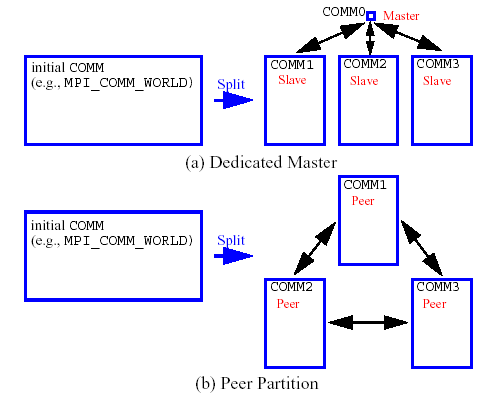
\includegraphics[width=70mm]{images/comm_partitioning}
  \caption{Communicator partitioning models.}
  \label{parallel:figure01}
\end{figure}

\subsubsection{Scheduling}\label{parallel:SLP:message:sched}

The following scheduling approaches are available within a level of
message passing parallelism:

\begin{itemize}
% TO DO: need a more descriptive term, e.g. single-point dedicated
% dynamic scheduling
\item \emph{Dynamic scheduling}: in the dedicated master model, the
  master processor manages a single processing queue and maintains a
  prescribed number of jobs (usually one) active on each slave. Once a
  slave server has completed a job and returned its results, the
  master assigns the next job to this slave. Thus, the job assignment
  on the master adapts to the job completion speed on the slaves. This
  provides a simple dynamic scheduler in that heterogeneous processor
  speeds and/or job durations are naturally handled, provided there
  are sufficient instances scheduled through the servers to balance
  the variation.  In the case of a peer partition, dynamic schedulers
  can also be employed, provided that peer 1 can employ nonblocking
  synchronization of its local evaluations.  This allows it to balance
  its local work with servicing job assignments and returns from the
  other peers.
\item \emph{Static scheduling}: if scheduling is statically determined
  at start-up, then no master processor is needed to direct traffic
  and a peer partitioning approach is applicable. If the static
  schedule is a good one (ideal conditions), then this approach will
  have superior performance. However, heterogeneity, when not known
  \emph{a priori}, can very quickly degrade performance since there is
  no mechanism to adapt.
\end{itemize}

%In addition, the following scheduling approach is provided by PICO for
%the scheduling of concurrent optimizations within the branch and bound
%minimizer:

%\begin{itemize}
% TO DO: this could become multipoint nondedicated dynamic scheduling
%\item \emph{Distributed scheduling}: in this approach, a peer
%  partition is used and each peer maintains a separate queue of
%  pending jobs. When one peer's queue is smaller than the other
%  queues, it requests work from its peers (prior to idleness). In this
%  way, it can adapt to heterogeneous conditions, provided there are
%  sufficient instances to balance the variation. Each partition
%  performs communication between computations, and no processors are
%  dedicated to scheduling. Furthermore, it distributes scheduling load
%  beyond a single processor, which can be important for large numbers
%  of concurrent jobs (whose scheduling might overload a single master)
%  or for fault tolerance (avoiding a single point of failure).
%  However, it involves relatively complicated logic and additional
%  communication for queue status and job migration, and its
%  performance is not always superior since a partition can become
%  work-starved if its peers are locked in computation (Note: this
%  logic can be somewhat simplified if a separate thread can be created
%  for communication and migration of jobs).
%\end{itemize}

Message passing schedulers may be used for managing concurrent
sub-iterator executions within a meta-iterator, concurrent evaluations
within an iterator, or concurrent analyses within an evaluation.  In
the former and latter cases, the message passing scheduler is
currently restricted to blocking synchronization, in that all jobs in
the queue are completed before exiting the scheduler and returning the
set of results to the algorithm. Nonblocking message-passing
scheduling is supported for the iterator--evaluation concurrency level
in support of fully asynchronous algorithms (e.g.,
\texttt{asynch\_pattern\_search} and \texttt{coliny\_pattern\_search})
that avoid synchronization points that can harm scaling.

Message passing is also used within a fine-grained parallel simulation
code, although this is separate from Dakota's capabilities (Dakota
may, at most, pass a communicator partition to the simulation).  The
``Message Passing'' column in Table~\ref{parallel:table01} summarizes
these capabilities.

\subsubsection{Message Passing Example}\label{parallel:SLP:message:ex}

Revisiting the test file \texttt{dakota\_dace.in}, Dakota will now
compute the 49 orthogonal array samples using a message passing
approach.  In this case, a parallel launch utility is used to execute
Dakota across multiple processors using syntax similar to the following:
\begin{small}
\begin{verbatim}
    mpirun -np 5 -machinefile machines dakota -i dakota_dace.in
\end{verbatim}
\end{small}

Since the asynchronous local parallelism will not be used, the
interface specification does not include the \texttt{asynchronous}
keyword and would appear similar to:
\begin{small}
\begin{verbatim}
    interface,
            system
              analysis_driver = 'text_book'
\end{verbatim}
\end{small}

The relevant excerpts from the Dakota output for a dedicated master
partition and dynamic schedule, the default when the maximum concurrency
(49) exceeds the available capacity (5), would appear similar to the
following:
\begin{small}
\begin{verbatim}
    Running MPI Dakota executable in parallel on 5 processors.
    -----------------------------------------------------------------------------
    DAKOTA parallel configuration:
    
    Level                       num_servers    procs_per_server    partition
    -----                       -----------    ----------------    ---------
    concurrent evaluations           5                1            peer
    concurrent analyses	             1                1            peer
    multiprocessor analysis          1               N/A           N/A
    
    Total parallelism levels =   1 (1 dakota, 0 analysis)
    -----------------------------------------------------------------------------
    >>>>> Executing environment.
    
    >>>>> Running dace iterator.
    
    DACE method = 12 Samples = 49 Symbols = 7 Seed (user-specified) = 5
    
    ------------------------------
    Begin       I1 Evaluation    1
    ------------------------------
    (Asynchronous job 1 added to I1 queue)
    
    ------------------------------
    Begin       I1 Evaluation    2
    ------------------------------
    (Asynchronous job 2 added to I1 queue)
    
    <snip>
    
    ------------------------------
    Begin       I1 Evaluation   49
    ------------------------------
    (Asynchronous job 49 added to I1 queue)
    
    Blocking synchronize of 49 asynchronous evaluations
    Peer dynamic schedule: first pass assigning 4 jobs among 4 remote peers
    Peer 1 assigning I1 evaluation 1 to peer 2
    Peer 1 assigning I1 evaluation 2 to peer 3
    Peer 1 assigning I1 evaluation 3 to peer 4
    Peer 1 assigning I1 evaluation 4 to peer 5
    Peer dynamic schedule: first pass launching 1 local jobs
    Initiating I1 evaluation 5
    text_book /tmp/file5LRsBu /tmp/fileT2mS65 &
    Peer dynamic schedule: second pass scheduling 44 remaining jobs
    Initiating I1 evaluation 5
    text_book /tmp/file5LRsBu /tmp/fileT2mS65 &
    Peer dynamic schedule: second pass scheduling 44 remaining jobs
    I1 evaluation 5 has completed
    Initiating I1 evaluation 6
    text_book /tmp/fileZJaODH /tmp/filewoUJaj &
    I1 evaluation 2 has returned from peer server 3
    Peer 1 assigning I1 evaluation 7 to peer 3
    I1 evaluation 4 has returned from peer server 5
    
    <snip>
    
    I1 evaluation 46 has returned from peer server 2
    I1 evaluation 49 has returned from peer server 5
    <<<<< Function evaluation summary (I1): 49 total (49 new, 0 duplicate)
    
    <<<<< Iterator dace completed.
\end{verbatim}
\end{small}
where it is evident that each of the 49 jobs is first queued and then
a blocking synchronization is performed.  This synchronization uses a
dynamic scheduler that initiates five jobs, one on each of five evaluation
servers, and then replaces completing jobs with new ones until all 49 are 
complete.  It is important to note that job execution local to each of the 
four servers is synchronous.


\subsection{Hybrid Parallelism}\label{parallel:SLP:hybrid}

The asynchronous local approaches described in
Section~\ref{parallel:SLP:local} can be considered to rely on
\emph{external} scheduling mechanisms, since it is generally the
operating system or some external queue/load sharing software that
allocates jobs to processors. Conversely, the message-passing
approaches described in Section~\ref{parallel:SLP:message} rely on
\emph{internal} scheduling mechanisms to distribute work among
processors. These two approaches provide building blocks which can be
combined in a variety of ways to manage parallelism at multiple
levels. At one extreme, Dakota can execute on a single processor and
rely completely on external means to map all jobs to processors (i.e.,
using asynchronous local approaches). At the other extreme, Dakota can
execute on many processors and manage all levels of parallelism,
including the parallel simulations, using completely internal
approaches (i.e., using message passing at all levels as in
Figure~\ref{parallel:figure02}). While all-internal or all-external
approaches are common cases, many additional approaches exist between
the two extremes in which some parallelism is managed internally and
some is managed externally.

These combined approaches are referred to as \emph{hybrid}
parallelism, since the internal distribution of work based on
message-passing is being combined with external allocation using
asynchronous local approaches\footnote{The term ``hybrid parallelism''
is often used to describe the combination of MPI message passing and
OpenMP shared memory parallelism models.  This can be considered to be
a special case of the meaning here, as OpenMP is based on threads,
which is analagous to asynchronous local usage of the direct
simulation interface.}.  Figure~\ref{parallel:figure03} depicts the
asynchronous local, message-passing, and hybrid approaches for a
dedicated-master partition. Approaches (b) and (c) both use MPI
message-passing to distribute work from the master to the slaves, and
approaches (a) and (c) both manage asynchronous jobs local to a
processor. The hybrid approach (c) can be seen to be a combination of
(a) and (b) since jobs are being internally distributed to slave
servers through message-passing and each slave server is managing
multiple concurrent jobs using an asynchronous local approach. From a
different perspective, one could consider (a) and (b) to be special
cases within the range of configurations supported by (c). The hybrid
approach is useful for supercomputers that maintain a service/compute
node distinction and for supercomputers or networks of workstations
that involve clusters of symmetric multiprocessors (SMPs). In the
service/compute node case, concurrent multiprocessor simulations are
launched into the compute nodes from the service node partition. While
an asynchronous local approach from a single service node would be
sufficient, spreading the application load by running Dakota in
parallel across multiple service nodes results in better
performance~\cite{Eld00}. If the number of concurrent jobs to be
managed in the compute partition exceeds the number of available
service nodes, then hybrid parallelism is the preferred approach. In
the case of a cluster of SMPs (or network of multiprocessor
workstations), message-passing can be used to communicate between
SMPs, and asynchronous local approaches can be used within an
SMP. Hybrid parallelism can again result in improved performance,
since the total number of Dakota MPI processes is reduced in
comparison to a pure message-passing approach over all processors.

Hybrid schedulers may be used for managing concurrent evaluations
within an iterator or concurrent analyses within an evaluation.  In
the former case, blocking or nonblocking synchronization can be used,
whereas the latter case is restricted to blocking synchronization.
The ``Hybrid'' column in Table~\ref{parallel:table01} summarizes these
capabilities.

\subsubsection{Hybrid Example}\label{parallel:SLP:hybrid:ex}

Revisiting the test file \texttt{dakota\_dace.in}, Dakota will now
compute the 49 orthogonal array samples using a hybrid approach.  As
for the message passing case, a parallel launch utility is used to
execute Dakota across multiple processors:
\begin{small}
\begin{verbatim}
    mpirun -np 5 -machinefile machines dakota -i dakota_dace.in
\end{verbatim}
\end{small}

Since the asynchronous local parallelism will also be used, the
interface specification includes the \texttt{asynchronous}
keyword and appears similar to
\begin{small}
\begin{verbatim}
    interface,
            system asynchronous evaluation_concurrency = 2
              analysis_driver = 'text_book'
\end{verbatim}
\end{small}
In the hybrid case, the specification of the desired concurrency level
must be included, since the default is no longer all available (as it
is for asynchronous local parallelism).  Rather the default is to employ
message passing parallelism, and hybrid parallelism is only available
through the specification of asynchronous concurrency greater than one.

The relevant excerpts of the Dakota output for a peer partition and dynamic schedule
, the default when the maximum concurrency
(49) exceeds the maximum available capacity (10), would appear similar
to the following:
\begin{small}
\begin{verbatim}
    Running MPI Dakota executable in parallel on 5 processors.
    
    -----------------------------------------------------------------------------
    DAKOTA parallel configuration:
    
    Level			num_servers    procs_per_server    partition
    -----			-----------    ----------------    ---------
    concurrent evaluations           5                1            peer
    concurrent analyses              1                1            peer
    multiprocessor analysis          1               N/A           N/A
    
    Total parallelism levels =   1 (1 dakota, 0 analysis)
    -----------------------------------------------------------------------------
    
    >>>>> Executing environment.
    
    >>>>> Running dace iterator.
    
    DACE method = 12 Samples = 49 Symbols = 7 Seed (user-specified) = 5
    
    ------------------------------
    Begin       I1 Evaluation    1
    ------------------------------
    (Asynchronous job 1 added to I1 queue)
    
    ------------------------------
    Begin       I1 Evaluation    2
    ------------------------------
    (Asynchronous job 2 added to I1 queue)
    
    <snip>
    
    Blocking synchronize of 49 asynchronous evaluations
    Peer dynamic schedule: first pass assigning 8 jobs among 4 remote peers
    Peer 1 assigning I1 evaluation 1 to peer 2
    Peer 1 assigning I1 evaluation 2 to peer 3
    Peer 1 assigning I1 evaluation 3 to peer 4
    Peer 1 assigning I1 evaluation 4 to peer 5
    Peer 1 assigning I1 evaluation 6 to peer 2
    Peer 1 assigning I1 evaluation 7 to peer 3
    Peer 1 assigning I1 evaluation 8 to peer 4
    Peer 1 assigning I1 evaluation 9 to peer 5
    Peer dynamic schedule: first pass launching 2 local jobs
    Initiating I1 evaluation 5
    text_book /tmp/fileJU1Ez2 /tmp/fileVGZzEX &
    Initiating I1 evaluation 10
    text_book /tmp/fileKfUgKS /tmp/fileMgZXPN &
    Peer dynamic schedule: second pass scheduling 39 remaining jobs
    
    <snip>
    
    I1 evaluation 49 has completed
    I1 evaluation 43 has returned from peer server 2
    I1 evaluation 44 has returned from peer server 3
    I1 evaluation 48 has returned from peer server 4
    I1 evaluation 47 has returned from peer server 2
    I1 evaluation 45 has returned from peer server 3
    <<<<< Function evaluation summary (I1): 49 total (49 new, 0 duplicate)
    
    <<<<< Iterator dace completed.
\end{verbatim}
\end{small}
where it is evident that each of the 49 jobs is first queued and then
a blocking synchronization is performed.  This synchronization uses a
dynamic scheduler that initiates ten jobs, two on each of five evaluation
servers, and then replaces completing jobs with new
ones until all 49 are complete.  It is important to note that job
execution local to each of the four servers is asynchronous.

\section{Multilevel parallelism} \label{parallel:MLP}


Parallel computers within the Department of Energy national
laboratories have achieved nearly 20 quadrillion ($10^{15}$) floating point
operations per second (20 petaFLOPS) in Linpack benchmarks. Planning
for "exascale" systems, rated at 1000 petaFLOPS, is well underway. 
This performance is achieved through the use of massively parallel (MP)
processing using $O[10^{5}-10^{6}]$ processors. In order to harness
the power of these machines for performing design, uncertainty
quantification, and other systems analyses, parallel algorithms are
needed which are scalable to thousands of processors.

Dakota supports an open-ended number of levels of nested parallelism
which, as described in Section~\ref{parallel:overview}, can be
categorized into three types of concurrent job scheduling and four
types of parallelism: (a) concurrent iterators within a meta-iterator
(scheduled by Dakota), (b) concurrent function evaluations within each
iterator (scheduled by Dakota), (c) concurrent analyses within each
function evaluation (scheduled by Dakota), and (d) multiprocessor
analyses (work distributed by a parallel analysis code).  In
combination, these parallelism levels can minimize efficiency losses
and achieve near linear scaling on MP computers.  Types (a) and (b)
are classified as algorithmic coarse-grained parallelism, type (c) is
function evaluation coarse-grained parallelism, and type (d) is
function evaluation fine-grained parallelism (see
Section~\ref{parallel:overview:cat}). Algorithmic fine-grained
parallelism is not currently supported in Dakota, although this 
picture is rapidly evolving. 
%the development of large-scale parallel SAND techniques is an ongoing
%research focus~\cite{Bar01b}.

A particular application may support one or more of these parallelism
types, and Dakota provides for convenient selection and combination of
multiple levels. If multiple types of parallelism can be exploited,
then the question may arise as to how the amount of parallelism at
each level should be selected so as to maximize the overall parallel
efficiency of the study. For performance analysis of multilevel
parallelism formulations and detailed discussion of these issues,
refer to~\cite{Eld00}.  In many cases, \emph{the user may simply
  employ Dakota's automatic parallelism configuration facilities,}
which implement the recommendations from the aforementioned paper.

Figure~\ref{fig:mlp_scaling} shows typical fixed-size scaling
performance using a modified version of the extended
\texttt{text\_book} problem (see Section~\ref{additional:textbook}).
Three levels of parallelism (concurrent evaluations within an
iterator, concurrent analyses within each evaluation, and
multiprocessor analyses) are exercised within a modest partition of
processors (circa year 2000).  Despite the use of a fixed problem size
and the presence of some idleness within the scheduling at multiple
levels, the efficiency is still reasonably high\footnote{Note that
  overhead is reduced in these scaling studies by deactivating the
  evaluation cache and restart file logging.}.  Greater efficiencies
are obtainable for scaled speedup studies (or for larger problems in
fixed-size studies) and for problems optimized for minimal scheduler
idleness (by, e.g., managing all concurrency in as few scheduling
levels as possible).  Note that speedup and efficiency are measured
relative to the case of a single instance of a multiprocessor
analysis, since it was desired to investigate the effectiveness of the
Dakota schedulers independent from the efficiency of the parallel
analysis.
\begin{figure}[ht]
  \centering
  \subfigure[Relative speedup.]
    {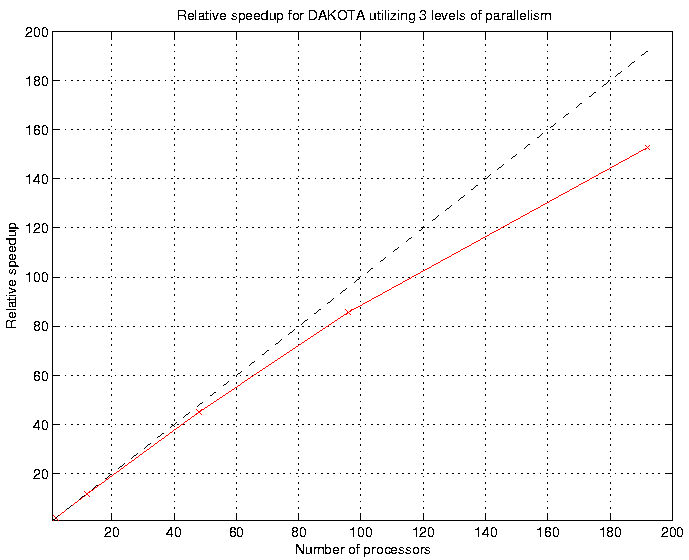
\includegraphics[width=.45\textwidth]{images/mss_rel_speedup_3lev_determ}}
  \subfigure[Relative efficiency.]
    {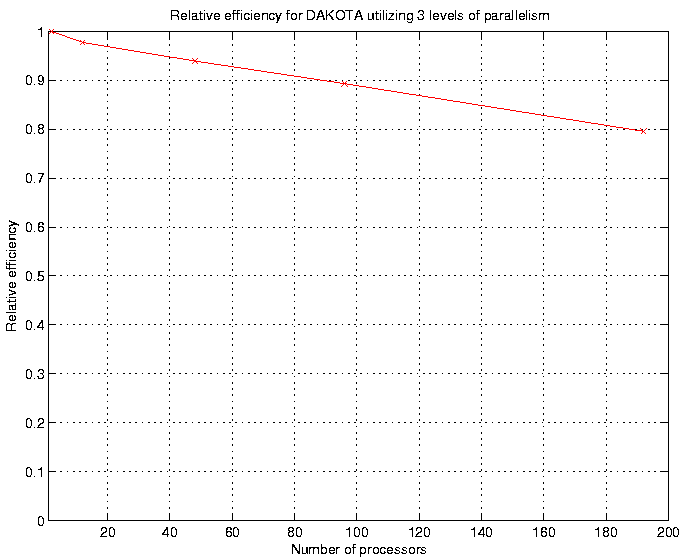
\includegraphics[width=.45\textwidth]{images/mss_rel_eff_3lev_determ}}
  \caption{Fixed-size scaling results for three levels of parallelism.}
  \label{fig:mlp_scaling}
% The 2 processor run uses a 1/1/1/2 configuration and is as small as can be
% fairly compared for the same level of fine-grained simulation.  The 12, 48,
% 96, and 192 processor runs use 3 levels of parallelism in a 1/eval_srv/3/2
% configuration with eval_srv = 2, 8, 16, and 32, respectively.
\end{figure}

\subsection{Asynchronous Local Parallelism}\label{parallel:MLP:local}

In most cases, the use of asynchronous local parallelism is the
termination point for multilevel parallelism, in that any level of
parallelism lower than an asynchronous local level will be serialized
(see discussion in Section~\ref{parallel:MLP:hybrid}).  The exception
to this rule is reforking of forked processes for concurrent analyses
within forked evaluations.  In this case, a new process is created
using fork for one of several concurrent evaluations; however, the new
process is not replaced immediately using exec.  Rather, the new
process is reforked to create additional child processes for executing
concurrent analyses within each concurrent evaluation process.  This
capability is not supported by system calls and provides one of the
key advantages to using fork over system (see
Section~\ref{interfaces:which}).

\subsection{Message Passing Parallelism}\label{parallel:MLP:message}

%\subsection{Communicator partitioning}
%   Lowest level supports single-level options above
\subsubsection{Partitioning of levels}\label{parallel:MLP:message:partitioning}

Dakota uses MPI communicators to identify groups of processors. The
global \texttt{MPI\_COMM\_WORLD} communicator provides the total set
of processors allocated to the Dakota run. \texttt{MPI\_COMM\_WORLD}
can be partitioned into new intra-communicators which each define a
set of processors to be used for a multiprocessor server. Each of
these servers may be further partitioned to nest one level of
parallelism within the next. At the lowest parallelism level, these
intra-communicators can be passed into a simulation for use as the
simulation's computational context, provided that the simulation has
been designed, or can be modified, to be modular on a communicator
(i.e., it does not assume ownership of \texttt{MPI\_COMM\_WORLD}). New
intra-communicators are created with the \texttt{MPI\_Comm\_split}
routine, and in order to send messages between these
intra-communicators, new inter-communicators are created with calls to
\texttt{MPI\_Intercomm\_create}. %To minimize overhead, Dakota creates
%new intra- and inter-communicators only when the parent communicator
%provides insufficient context for the scheduling at a particular level. 
Multiple parallel configurations (containing a set of communicator
partitions) are allocated for use in studies with multiple iterators
and models (e.g., 16 servers of 64 processors each could be used for
iteration on a lower fidelity model, followed by two servers of 512
processors each for subsequent iteration on a higher fidelity model),
and can be alternated at run time.  Each of the parallel
configurations are allocated at object construction time and are
reported at the beginning of the Dakota output.

Each tier within Dakota's nested parallelism hierarchy can use the
dedicated master and peer partition approaches described in
Section~\ref{parallel:SLP:message:part}. To recursively partition the
subcommunicators of Figure~\ref{parallel:figure01},
\texttt{COMM1/2/3} in the dedicated master or peer partition case
would be further subdivided using the appropriate partitioning model
for the next lower level of parallelism.


\subsubsection{Scheduling within levels}\label{parallel:MLP:message:scheduling}

\begin{figure}[ht]
  \centering
  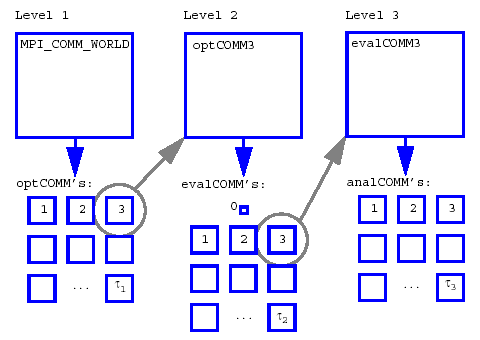
\includegraphics[width=60mm]{images/recursive_partitioning}
  \caption{Recursive partitioning for nested parallelism.}
  \label{parallel:figure02}
\end{figure}

Dakota is designed to allow the freedom to configure each parallelism
level with either the dedicated master partition/dynamic scheduling
combination or the peer partition/static scheduling combination. In
addition, the iterator-evaluation level supports a peer partition/dynamic 
scheduling option, and certain external libraries may provide custom options.
%(e.g., PICO supports distributed scheduling in peer partitions).
As an
example, Figure~\ref{parallel:figure02} shows a case in which a branch
and bound meta-iterator employs peer partition/distributed scheduling 
at level 1, each optimizer partition employs concurrent function
evaluations in a dedicated master partition/dynamic scheduling model at
level 2, and each function evaluation partition employs concurrent
multiprocessor analyses in a peer partition/static scheduling model at
level 3. In this case, \texttt{MPI\_COMM\_WORLD} is subdivided into
\texttt{optCOMM1/2/3/.../$\tau_{1}$}, each \texttt{optCOMM} is further
subdivided into \texttt{evalCOMM0} (master) and
\texttt{evalCOMM1/2/3/.../$\tau_{2}$} (slaves), and each slave
\texttt{evalCOMM} is further subdivided into
\texttt{analCOMM1/2/3/.../$\tau_{3}$}.  Logic for selecting the
$\tau_i$ that maximize overall efficiency is discussed in~\cite{Eld00}.


\subsection{Hybrid Parallelism}\label{parallel:MLP:hybrid}

Hybrid parallelism approaches can take several forms when used in the
multilevel parallel context. A conceptual boundary can be considered
to exist for which all parallelism above the boundary is managed
internally using message-passing and all parallelism below the
boundary is managed externally using asynchronous local approaches.
Hybrid parallelism approaches can then be categorized based on whether
this boundary between internal and external management occurs within a
parallelism level (\emph{intra-level}) or between two parallelism
levels (\emph{inter-level}). In the intra-level case, the jobs for the
parallelism level containing the boundary are scheduled using a hybrid
scheduler, in which a capacity multiplier is used for the number of
jobs to assign to each server. Each server is then responsible for
concurrently executing its capacity of jobs using an asynchronous
local approach. In the inter-level case, one level of parallelism
manages its parallelism internally using a message-passing approach
and the next lower level of parallelism manages its parallelism
externally using an asynchronous local approach. That is, the jobs for
the higher level of parallelism are scheduled using a standard
message-passing scheduler, in which a single job is assigned to each
server. However, each of these jobs has multiple components, as
managed by the next lower level of parallelism, and each server is
responsible for executing these sub-components concurrently using an
asynchronous local approach.

For example, consider a multiprocessor Dakota run which involves an
iterator scheduling a set of concurrent function evaluations across a
cluster of SMPs. A hybrid parallelism approach will be applied in
which message-passing parallelism is used between SMPs and
asynchronous local parallelism is used within each SMP. In the hybrid
intra-level case, multiple function evaluations would be scheduled to
each SMP, as dictated by the capacity of the SMPs, and each SMP would
manage its own set of concurrent function evaluations using an
asynchronous local approach. Any lower levels of parallelism would be
serialized. In the hybrid inter-level case, the function evaluations
would be scheduled one per SMP, and the analysis components within
each of these evaluations would be executed concurrently using
asynchronous local approaches within the SMP. Thus, the distinction
can be viewed as whether the concurrent jobs on each server in
Figure~\ref{parallel:figure03}c reflect the same level of parallelism
as that being scheduled by the master (intra-level) or one level of
parallelism below that being scheduled by the master (inter-level).


\section{Capability Summary}\label{parallel:summary}


Table~\ref{parallel:table01} shows a matrix of the supported job
management approaches for each of the parallelism levels, with
supported simulation interfaces and synchronization approaches shown
in parentheses. The concurrent iterator and multiprocessor analysis
parallelism levels can only be managed with message-passing
approaches. In the former case, this is due to the fact that a
separate process or thread for an iterator is not currently supported.
The latter case reflects a finer point on the definition of external
parallelism management. While a multiprocessor analysis can most
certainly be launched (e.g., using \texttt{mpirun}/\texttt{yod}) from
one of Dakota's analysis drivers, resulting in a parallel analysis
external to Dakota (which is consistent with asynchronous local and
hybrid approaches), this parallelism is not visible to Dakota and
therefore does not qualify as parallelism that Dakota manages (and
therefore is not included in Table~\ref{parallel:table01}). The
concurrent evaluation and analysis levels can be managed either with
message-passing, asynchronous local, or hybrid techniques, with the
exceptions that the direct interface does not support asynchronous
operations (asynchronous local or hybrid) at either of these levels
and the system call interface does not support asynchronous operations
(asynchronous local or hybrid) at the concurrent analysis level. The
direct interface restrictions are present since multithreading in not
yet supported and the system call interface restrictions result from
the inability to manage concurrent analyses within a nonblocking
function evaluation system call.  Finally, nonblocking synchronization
is only supported at the concurrent function evaluation level,
although it spans asynchronous local, message passing, and hybrid
parallelism options.

\begin{table}
  \centering
  \caption{Support of job management approaches within parallelism levels.
  Shown in parentheses are supported simulation interfaces and supported
  synchronization approaches.}
  \label{parallel:table01}\vspace{2mm}
  \begin{tabular}{c||c|c|c|}
    %\hline
    \textbf{Parallelism Level} & \textbf{Asynchronous Local} &
    \textbf{Message Passing} & \textbf{Hybrid} \\
    \hline \hline
    concurrent iterators within a & & \textbf{X}      & \\
    meta-iterator or nested model & & (blocking synch) & \\
    \hline
    concurrent function evaluations & \textbf{X} & \textbf{X} & \textbf{X} \\
    within an iterator          & (system, fork) & (system, fork, direct) &
    (system, fork) \\
    & (blocking, nonblocking) & (blocking, nonblocking) &
      (blocking, nonblocking) \\
    \hline
    concurrent analyses & \textbf{X} & \textbf{X} & \textbf{X} \\
    within a function evaluation & (fork only) & (system, fork, direct) &
    (fork only) \\
    & (blocking synch) & (blocking synch) & (blocking synch) \\
    \hline
    fine-grained parallel analysis & & \textbf{X} & \\
    \hline
  \end{tabular}
\end{table}


\section{Running a Parallel Dakota Job}\label{parallel:running}


Section~\ref{parallel:SLP} provides a few examples of serial and
parallel execution of Dakota using asynchronous local, message
passing, and hybrid approaches to single-level parallelism.  The
following sections provides a more complete discussion of the parallel
execution syntax and available specification controls.


\subsection{Single-processor execution}\label{parallel:running:single}

The command for running Dakota on a single-processor and exploiting
asynchronous local parallelism is the same as for running Dakota on a
single-processor for a serial study, e.g.:
\begin{small}
\begin{verbatim}
    dakota -i dakota.in > dakota.out
\end{verbatim}
\end{small}

See Section~\ref{tutorial:installation:running} for additional
information on single-processor command syntax.

\subsection{Multiprocessor execution}\label{parallel:running:multiprocessor}

Running a Dakota job on multiple processors requires the use of an
executable loading facility such as \texttt{mpirun}, \texttt{mpiexec},
\texttt{poe}, or \texttt{yod}.  On a network of workstations, the
\texttt{mpirun} script is commonly used to initiate a parallel Dakota
job, e.g.:
\begin{small}
\begin{verbatim}
    mpirun -np 12 dakota -i dakota.in > dakota.out
    mpirun -machinefile machines -np 12 dakota -i dakota.in > dakota.out
\end{verbatim}
\end{small}
where both examples specify the use of 12 processors, the former
selecting them from a default system resources file and the latter
specifying particular machines in a machine file (see~\cite{Gro96} for
details).

On a massively parallel computer, the familiar mpirun/mpiexec options
may be replaced with other launch scripts as dictated by the
particular software stack, e.g.:
\begin{small}
\begin{verbatim}
    yod -sz 512 dakota -i dakota.in > dakota.out
\end{verbatim}
\end{small}

In each of these cases, MPI command line arguments are used by MPI
(extracted first in the call to \texttt{MPI\_Init}) and Dakota command
line arguments are used by Dakota (extracted second by Dakota's
command line handler). %An issue that can arise with these command line
%arguments is that the mpirun script distributed with MPICH has been
%observed to have problems with certain file path specifications (e.g.,
%a relative path such as ``\texttt{../some\_file}''). These path
%problems are most easily resolved by using local linkage (all
%referenced files or soft links to these files appear in the same
%directory).

Finally, when running on computer resources that employ NQS/PBS 
batch schedulers, the single-processor \texttt{dakota} command syntax or the
multiprocessor \texttt{mpirun} command syntax might be contained
within an executable script file which is submitted to the batch
queue. For example, a command
\begin{small}
\begin{verbatim}
    qsub -l size=512 run_dakota
\end{verbatim}
\end{small}

could be submitted to a PBS queue for execution. The NQS syntax is 
similar:
\begin{small}
\begin{verbatim}
    qsub -q snl -lP 512 -lT 6:00:00 run_dakota
\end{verbatim}
\end{small}

These commands allocate 512 compute nodes for the study, and execute
the \texttt{run\_dakota} script on a service node. If this script
contains a single-processor \texttt{dakota} command, then Dakota will
execute on a single service node from which it can launch parallel
simulations into the compute nodes using analysis drivers that contain
\texttt{yod} commands (any \texttt{yod} executions occurring at any
level underneath the \texttt{run\_dakota} script are mapped to the 512
compute node allocation). If the script submitted to \texttt{qsub}
contains a multiprocessor \texttt{mpirun} command, then Dakota will
execute across multiple service nodes so that it can spread the
application load in either a message-passing or hybrid parallelism
approach. Again, analysis drivers containing \texttt{yod} commands
would be responsible for utilizing the 512 compute nodes. And,
finally, if the script submitted to \texttt{qsub} contains a
\texttt{yod} of the \texttt{dakota} executable, then Dakota will
execute directly on the compute nodes and manage all of the
parallelism internally (note that a \texttt{yod} of this type without
a \texttt{qsub} would be mapped to the interactive partition, rather
than to the batch partition).

Not all supercomputers employ the same model for service/compute
partitions or provide the same support for tiling of concurrent
multiprocessor simulations within a single NQS/PBS allocation.  For
this reason, templates for parallel job configuration are being
catalogued within {\tt Dakota/examples/script\_interfaces} and 
\texttt{Dakota/examples/parallelism} (in the software
distributions) that are intended to provide guidance for individual
machine idiosyncrasies.

Dakota relies on hints from the runtime environment and command
line arguments to detect when it has been launched in parallel. Due to 
the large number of HPC vendors and MPI implementations, parallel launch
is not always detected properly. A parallel launch is indicated
by the status message 
\begin{small}
\begin{verbatim}
  Running MPI Dakota executable in parallel on N processors. 
\end{verbatim}
\end{small}

which is written to the console near the beginning of the Dakota run.

Beginning with release 6.5, if Dakota incorrectly detects a parallel launch, 
automatic detection can be overriden by setting the environment variable 
\texttt{DAKOTA\_RUN\_PARALLEL}. If the first character is set to \texttt{1}, 
\texttt{t}, or \texttt{T}, Dakota will configure itself to run in parallel.
If the variable exists but is set to anything else, Dakota will configure 
itself to run in serial mode.

\section{Specifying Parallelism}\label{parallel:spec}

Given an allotment of processors, Dakota contains logic based on the
theoretical work in~\cite{Eld00} to automatically determine an efficient
parallel configuration, consisting of partitioning and scheduling
selections for each of the parallelism levels. This logic accounts for
problem size, the concurrency supported by particular iterative
algorithms, and any user inputs or overrides. 

Concurrency is pushed up for most parallelism levels. That is,
available processors will be assigned to concurrency at the higher
parallelism levels first as we partition from the top down.  If more
processors are available than needed for concurrency at a level, then
the server size is increased to support concurrency in the next lower
level of parallelism.  This process is continued until all available
processors have been assigned. These assignments can be overridden by
the user by specifying a number of servers, processors per server, or
both, for the concurrent iterator, evaluation, and analysis
parallelism levels. For example, if it is desired to parallelize
concurrent analyses within each function evaluation, then an
\texttt{evaluation\_servers = 1} override would serialize the
concurrent function evaluations level and ensure processor
availability for concurrent analyses.

The exception to this push up of concurrency occurs for
concurrent-iterator parallelism levels, since iterator executions tend
to have high variability in duration whenever they utilize feedback of
results.  For these levels, concurrency is pushed down since it is
generally best to serialize the levels with the highest job variation
and exploit concurrency elsewhere.

Partition type (master or peer) may also be specified for each level, 
and peer scheduling type (dynamic or static) may be specified at the 
level of evaluation concurrency. However, these selections may be 
overridden by Dakota if they are inconsistent with the number of 
user-requested servers, processors per server, and available processors.

In the following sections, the user inputs and overrides are
described, followed by specification examples for single and
multi-processor Dakota executions.

\subsection{The interface specification}\label{parallel:spec:interface}

Specifying parallelism within an interface can involve the use of the
\texttt{asynchronous}, \texttt{evaluation\_concurrency}, and
\texttt{analysis\_concurrency} keywords to specify concurrency local
to a processor (i.e., asynchronous local parallelism). This
\texttt{asynchronous} specification has dual uses:

\begin{itemize}
\item When running Dakota on a single-processor, the
  \texttt{asynchronous} keyword specifies the use of asynchronous
  invocations local to the processor (these jobs then rely on external
  means to be allocated to other processors). The default behavior is
  to simultaneously launch all function evaluations available from the
  iterator as well as all available analyses within each function
  evaluation. In some cases, the default behavior can overload a
  machine or violate a usage policy, resulting in the need to limit
  the number of concurrent jobs using the
  \texttt{evaluation\_concurrency} and \texttt{analysis\_concurrency}
  specifications. 

\item When executing Dakota across multiple processors and managing
  jobs with a message-passing scheduler, the \texttt{asynchronous}
  keyword specifies the use of asynchronous invocations local to each
  server processor, resulting in a hybrid parallelism approach (see
  Section~\ref{parallel:SLP:hybrid}). In this case, the default
  behavior is one job per server, which must be overridden with an
  \texttt{evaluation\_concurrency} specification and/or an
  \texttt{analysis\_concurrency} specification. When a hybrid
  parallelism approach is specified, the capacity of the servers (used
  in the automatic configuration logic) is defined as the number of
  servers times the number of asynchronous jobs per server.
\end{itemize}

In both cases, the scheduling of local evaluations is dynamic by
default, but may be explicitly selected or overriden using
\texttt{local\_evaluation\_scheduling dynamic} or \texttt{static}.

In addition, \texttt{evaluation\_servers},
\texttt{processors\_per\_evaluation}, and
\texttt{evaluation\_scheduling} keywords can be used to override the
automatic parallel configuration for concurrent function
evaluations. Evaluation scheduling may be selected to be
\texttt{master} or \texttt{peer}, where the latter must be further
specified to be \texttt{dynamic} or \texttt{static}. 

To override the automatic parallelism configuration for concurrent
analyses, the \texttt{analysis\_servers} and
\texttt{analysis\_scheduling} keywords may be specified, and the
\texttt{processors\_per\_analysis} keyword can be used to override the
automatic parallelism configuration for the size of multiprocessor
analyses used in a direct function simulation interface. Scheduling
options for this level include \texttt{master} or \texttt{peer}, where
the latter is static (no dynamic peer option supported).  Each of
these keywords appears as part of the interface commands specification
in the Dakota Reference Manual~\cite{RefMan}.

\subsection{The meta-iterator and nested model specifications}\label{parallel:spec:meta}

To specify concurrency in sub-iterator executions within
meta-iterators and nested models, the \texttt{iterator\_servers},
\texttt{processors\_per\_iterator}, and \texttt{iterator\_scheduling}
keywords are used to override the automatic parallelism configuration.
For this level, the available scheduling options are \texttt{master}
or \texttt{peer}, where the latter is static (no dynamic peer option
supported).  See the method and model commands specification in the
Dakota Reference Manual~\cite{RefMan} for additional details.

\subsection{Single-processor Dakota specification}\label{parallel:spec:single}

Specifying a single-processor Dakota job that exploits parallelism
through asynchronous local approaches (see
Figure~\ref{parallel:figure03}a) requires inclusion of the
\texttt{asynchronous} keyword in the interface specification. Once the
input file is defined, single-processor Dakota jobs are executed using
the command syntax described previously in
Section~\ref{parallel:running:single}.

\subsubsection{Example 1}\label{parallel:spec:single:example1}

For example, the following specification runs an NPSOL optimization
which will perform asynchronous finite differencing:
\begin{small}
\begin{verbatim}
    method,
            npsol_sqp

    variables,
            continuous_design = 5
              initial_point  0.2  0.05 0.08 0.2  0.2
              lower_bounds   0.15 0.02 0.05 0.1  0.1
              upper_bounds   2.0  2.0  2.0  2.0  2.0

    interface,
            system,
              asynchronous
              analysis_drivers = 'text_book'

    responses,
            num_objective_functions = 1
            num_nonlinear_inequality_constraints = 2
            numerical_gradients
              interval_type central
              method_source dakota
              fd_gradient_step_size = 1.e-4
            no_hessians
\end{verbatim}
\end{small}

Note that \texttt{method\_source} \texttt{dakota} selects Dakota's
internal finite differencing routine so that the concurrency in finite
difference offsets can be exploited. In this case, central
differencing has been selected and 11 function evaluations (one at the
current point plus two offsets in each of five variables) can be
performed simultaneously for each NPSOL response request. These 11
evaluations will be launched with system calls in the background and
presumably assigned to additional processors through the operating
system of a multiprocessor compute server or other comparable method.
The concurrency specification may be included if it is necessary to
limit the maximum number of simultaneous evaluations. For example, if
a maximum of six compute processors were available, the command
\begin{small}
\begin{verbatim}
    evaluation_concurrency = 6
\end{verbatim}
\end{small}
could be added to the \texttt{asynchronous} specification within the
\texttt{interface} keyword from the preceding example.

\subsubsection{Example 2}\label{parallel:spec:single:example2}

If, in addition, multiple analyses can be executed concurrently within
a function evaluation (e.g., from multiple load cases or disciplinary
analyses that must be evaluated to compute the response data set),
then an input specification similar to the following could be used:
\begin{small}
\begin{verbatim}
    method,
            npsol_sqp

    variables,
            continuous_design = 5
              initial_point  0.2  0.05 0.08 0.2  0.2
              lower_bounds   0.15 0.02 0.05 0.1  0.1
              upper_bounds   2.0  2.0  2.0  2.0  2.0

    interface,
            fork
              asynchronous
                evaluation_concurrency = 6
                analysis_concurrency = 3
              analysis_drivers = 'text_book1' 'text_book2' 'text_book3'

    responses,
            num_objective_functions = 1
            num_nonlinear_inequality_constraints = 2
            numerical_gradients
              method_source dakota
              interval_type central
              fd_gradient_step_size = 1.e-4
            no_hessians
\end{verbatim}
\end{small}

In this case, the default concurrency with just an
\texttt{asynchronous} specification would be all 11 function
evaluations and all 3 analyses, which can be limited by the
\texttt{evaluation\_concurrency} and \texttt{analysis\_concurrency}
specifications. The input file above limits the function evaluation
concurrency, but not the analysis concurrency (a specification of 3 is
the default in this case and could be omitted). Changing the input to
\texttt{evaluation\_concurrency = 1} would serialize the function
evaluations, and changing the input to \texttt{analysis\_concurrency = 1}
would serialize the analyses.

\subsection{Multiprocessor Dakota specification}\label{parallel:spec:multi}

In multiprocessor executions, server evaluations are synchronous
(Figure~\ref{parallel:figure03}b) by default and the
\texttt{asynchronous} keyword is only used if a hybrid parallelism
approach (Figure~\ref{parallel:figure03}c) is desired. Multiprocessor
Dakota jobs are executed using the command syntax described previously
in Section~\ref{parallel:running:multiprocessor}.

\subsubsection{Example 3}\label{parallel:spec:multi:example3}

To run Example 1 using a message-passing approach, the
\texttt{asynchronous} keyword would be removed (since the servers will
execute their evaluations synchronously), resulting in the following
interface specification:
\begin{small}
\begin{verbatim}
    interface,
            system,
              analysis_drivers = 'text_book'
\end{verbatim}
\end{small}

Running Dakota on 4 processors (syntax: \texttt{mpirun -np 4 dakota -i
  dakota.in}) would result in the following parallel configuration
report from the Dakota output:
\begin{small}
\begin{verbatim}
    -----------------------------------------------------------------------------
    Dakota parallel configuration:

    Level                   num_servers    procs_per_server    partition
    -----                   -----------    ----------------    ---------
    concurrent evaluations       4                1            peer
    concurrent analyses          1                1            peer
    multiprocessor analysis      1               N/A           N/A

    Total parallelism levels =   1 (1 dakota, 0 analysis)
    -----------------------------------------------------------------------------
\end{verbatim}
\end{small}

In this case, a peer partition and dynamic scheduling algorithm are
automatically selected for the concurrent evaluations. If a dedicated
master is desired instead, then this logic could be overriden by adding
\texttt{evaluation\_scheduling master}:
\begin{small}
\begin{verbatim}
    interface,
            system,
              evaluation_scheduling master
              analysis_drivers = 'text_book'
\end{verbatim}
\end{small}

Running Dakota again on 4 processors (syntax: \texttt{mpirun -np 4
  dakota -i dakota.in}) would now result in this parallel
configuration report:
\begin{small}
\begin{verbatim}
    -----------------------------------------------------------------------------
    Dakota parallel configuration:

    Level                   num_servers    procs_per_server    partition
    -----                   -----------    ----------------    ---------
    concurrent evaluations       3                1            ded. master
    concurrent analyses          1                1            peer
    multiprocessor analysis      1               N/A           N/A

    Total parallelism levels =   1 (1 dakota, 0 analysis)
    -----------------------------------------------------------------------------
\end{verbatim}
\end{small}

Now the 11 jobs will be dynamically distributed among 3 slave servers,
under the control of 1 dedicated master.

As a related example, consider the case where each of the workstations
used in the parallel execution has multiple processors. In this case,
a hybrid parallelism approach which combines message-passing
parallelism with asynchronous local parallelism (see
Figure~\ref{parallel:figure03}c) would be a good choice. To specify
hybrid parallelism, one uses the same \texttt{asynchronous}
specification as was used for the single-processor examples, e.g.:
\begin{small}
\begin{verbatim}
    interface,
             system
               asynchronous evaluation_concurrency = 3
               analysis_drivers = `text_book'
\end{verbatim}
\end{small}

With 3 function evaluations concurrent on each server, the capacity of
a 4 processor Dakota execution (syntax: \texttt{mpirun -np 4 dakota -i
  dakota.in}) has increased to 12 evaluations. Since all 11 jobs can
now be scheduled in a single pass, a peer static scheduler is sufficient.

\begin{small}
\begin{verbatim}
    -----------------------------------------------------------------------------
    Dakota parallel configuration:

    Level                   num_servers    procs_per_server    partition
    -----                   -----------    ----------------    ---------
    concurrent evaluations       4                1            peer
    concurrent analyses          1                1            peer
    multiprocessor analysis      1               N/A           N/A

    Total parallelism levels =   1
    -----------------------------------------------------------------------------
\end{verbatim}
\end{small}

\subsubsection{Example 4}\label{parallel:spec:multi:example4}

To run Example 2 using a message-passing approach, the
\texttt{asynchronous} specification is again removed:
\begin{small}
\begin{verbatim}
    interface,
             fork
               analysis_drivers = `text_book1' `text_book2' `text_book3'
\end{verbatim}
\end{small}

Running this example on 6 processors (syntax: \texttt{mpirun -np 6
  dakota -i dakota.in}) would result in the following parallel
configuration report:
\begin{small}
\begin{verbatim}
    -----------------------------------------------------------------------------
    Dakota parallel configuration:

    Level                   num_servers    procs_per_server    partition
    -----                   -----------    ----------------    ---------
    concurrent evaluations       6                1            peer
    concurrent analyses          1                1            peer
    multiprocessor analysis      1               N/A           N/A

    Total parallelism levels =   1
    -----------------------------------------------------------------------------
\end{verbatim}
\end{small}

in which all of the processors have been assigned to support
evaluation concurrency due to the ``push up'' automatic configuration
logic. To assign some of the available processors to the concurrent 
analysis level, the following input could be used:
\begin{small}
\begin{verbatim}
    interface,
             fork
               analysis_drivers = `text_book1' `text_book2' `text_book3'
               evaluation_scheduling peer static
               evaluation_servers = 2
\end{verbatim}
\end{small}

which results in the following 2-level parallel configuration:
\begin{small}
\begin{verbatim}
    -----------------------------------------------------------------------------
    Dakota parallel configuration:

    Level                   num_servers    procs_per_server    partition
    -----                   -----------    ----------------    ---------
    concurrent evaluations       2                3            peer
    concurrent analyses          3                1            peer
    multiprocessor analysis      1               N/A           N/A

    Total parallelism levels =   2
    -----------------------------------------------------------------------------
\end{verbatim}
\end{small}

The six processors available have been split into two evaluation
servers of three processors each, where the three processors in each
evaluation server manage the three analyses, one per processor. Note that
without the scheduling override, a dedicated master partition at the 
evaluation level would have been chosen automatically, dividing
the six available processors into one evaluation server with three 
processors and another with two.

Next, consider the following 3-level parallel case, in which
\texttt{text\_book1}, \texttt{text\_book2}, and \texttt{text\_book3}
from the previous examples now execute on two processors each. In this
case, the \texttt{processors\_per\_analysis} keyword is added and the
\texttt{fork} interface is changed to a \texttt{direct} interface
since the fine-grained parallelism of the three simulations is managed
internally:
\begin{small}
\begin{verbatim}
    interface,
             direct
               analysis_drivers = `text_book1' `text_book2' `text_book3'
               evaluation_scheduling peer static
               evaluation_servers = 2
               processors_per_analysis = 2
\end{verbatim}
\end{small}

This results in the following parallel configuration for a 12
processor Dakota run \\
(syntax: \texttt{mpirun -np 12 dakota -i dakota.in}):
\begin{small}
\begin{verbatim}
    -----------------------------------------------------------------------------
    Dakota parallel configuration:

    Level                   num_servers    procs_per_server    partition
    -----                   -----------    ----------------    ---------
    concurrent evaluations       2                6            peer
    concurrent analyses          3                2            peer
    multiprocessor analysis      2               N/A           N/A

    Total parallelism levels =   3 (2 dakota, 1 analysis)
    -----------------------------------------------------------------------------
\end{verbatim}
\end{small}

An important point to recognize is that, since each of the parallel
configuration inputs has been tied to the interface specification up
to this point, these parallel configurations can be reallocated for
each interface in a multi-iterator/multi-model study. For example,
a Dakota execution on 40 processors might involve the following two
interface specifications:
\begin{small}
\begin{verbatim}
    interface,
            direct,
              id_interface = 'COARSE'
              analysis_driver = 'sim1'
              evaluation_scheduling peer dynamic
              processors_per_analysis = 5

    interface,
            direct,
              id_interface = 'FINE'
              analysis_driver = 'sim2'
              evaluation_scheduling peer dynamic
              processors_per_analysis = 10
\end{verbatim}
\end{small}

for which the coarse model would employ 8 evaluation servers of 5 
processors each and the fine model would employ 4 evaluation servers 
of 10 processors each.

Next, consider the following 4-level parallel case that employs the
Pareto set optimization meta-iterator. In this case,
\texttt{iterator\_servers} and \texttt{iterator\_scheduling peer}
requests are included in the method specification:
\begin{small}
\begin{verbatim}
    method,
             pareto_set
               iterator_servers = 2
               iterator_scheduling peer
               opt_method_pointer = 'NLP'
               random_weight_sets = 4
\end{verbatim}
\end{small}

Adding this \texttt{pareto\_set} method specification to the input file from 
the previous 12 processor example results in the following parallel configuration
for a 24 processor Dakota run \\
(syntax: \texttt{mpirun -np 24 dakota -i dakota.in}):
\begin{small}
\begin{verbatim}
    -----------------------------------------------------------------------------
    Dakota parallel configuration:

    Level                   num_servers    procs_per_server    partition
    -----                   -----------    ----------------    ---------
    concurrent iterators         2               12            peer
    concurrent evaluations       2                6            peer
    concurrent analyses          3                2            peer
    multiprocessor analysis      2               N/A           N/A

    Total parallelism levels =   4 (3 dakota, 1 analysis)
    -----------------------------------------------------------------------------
\end{verbatim}
\end{small}

Note that for this example, the parallel configuration is written to the
file \texttt{dakota.out.1} because of the use of concurrent iterators.

\subsubsection{Example 5}\label{parallel:spec:multi:example5}

As a final example, consider a multi-start optimization conducted on
384 processors. A job of this size must be submitted to
the batch queue, using syntax similar to:
\begin{small}
\begin{verbatim}
    qsub -q snl -lP 384 -lT 6:00:00 run_dakota
\end{verbatim}
\end{small}

where the \texttt{run\_dakota} script appears as
\begin{small}
\begin{verbatim}
    #!/bin/sh
    cd /scratch/<some_workdir>
    yod -sz 384 dakota -i dakota.in > dakota.out
\end{verbatim}
\end{small}

the interface specifications from the
\texttt{dakota.in} input file appears as
\begin{small}
\begin{verbatim}
    interface,
            direct,
              analysis_drivers = 'text_book1' 'text_book2' 'text_book3'
              evaluation_servers = 8
              evaluation_scheduling peer dynamic
              processors_per_analysis = 2
\end{verbatim}
\end{small}

and finally, an additional method section is added
\begin{small}
\begin{verbatim}

    method,
            multi_start
              method_pointer = 'CPS'
              iterator_servers = 8
              random_starts = 8
\end{verbatim}
\end{small}

The resulting parallel configuration is reported as
\begin{small}
\begin{verbatim}
    -----------------------------------------------------------------------------
    Dakota parallel configuration:

    Level                   num_servers    procs_per_server    partition
    -----                   -----------    ----------------    ---------
    concurrent iterators         8               48            peer
    concurrent evaluations       8                6            peer
    concurrent analyses          3                2            peer
    multiprocessor analysis      2               N/A           N/A

    Total parallelism levels =   4 (3 dakota, 1 analysis)
    -----------------------------------------------------------------------------
\end{verbatim}
\end{small}

Since the concurrency at each of the nested levels has a
multiplicative effect on the number of processors that can be
utilized, it is easy to see how large numbers of processors can be put
to effective use in reducing the time to reach a solution, even when,
as in this example, the concurrency per level is relatively low.


\section{Application Parallelism Use Cases}\label{parallel:application}

This section describes several common use cases for running Dakota on
parallel computing clusters with various combinations of Dakota and
application parallelism.  In three of the four cases addressed, the
application launched by Dakota is assumed MPI-enabled and run as an
independent parallel process. 

The {\tt examples/parallelism} folder in the Dakota installation includes
examples of the use cases. In all four, Dakota performs a vector parameter
on the "textbook" test function described in Section~\ref{additional:textbook}.
The application executed for serial demonstration is the {\tt text\_book} 
example driver, and for parallel execution, a modified version named 
{\tt text\_book\_simple\_par}. Both are located in Dakota's {\tt test} folder.
Dakota uses its fork interface to launch interface scripts written either in
Bash or Python, which include mock pre-processing to prepare application input,
application execution in serial or parallel, and post-processing of application
results to return to Dakota.

The combinations of Dakota and application parallelism are summarized
in Table~\ref{parallel:application:table01}.  In each case, $M$
denotes the total number of processors (or MPI tasks) allocated and $N$ 
denotes the number of processors used by a single application analysis.  
For most scenarios, Cases 1--3, where Dakota and the application jobs run
within a single cluster processor allocation (queued job), are
preferred.  However for particularly long-running or large jobs, or
platforms that not supporting the first scheduling modes, Case 4 may
be most appropriate.
\begin{table}
  \centering
  \caption{Cases for Dakota and application-level parallelism with $M$
  available processors and each application job requiring $N$
  processors.  Cases 1--3 assume that Dakota and any application runs
  will execute wholly within a single scheduled job, whereas Case 4 is
  relevant when analysis jobs must be individually submitted to a
  scheduler.}
  \newcolumntype{L}[1]{>{\centering\arraybackslash}m{#1}}
  \label{parallel:application:table01}\vspace{2mm}
  \begin{tabular}{c|L{2cm}|c|c|L{7.5cm}}
    {\bf Case} & {\bf Name } & {\bf Dakota} & {\bf Application} & {\bf Notes} \\
    \hline 1 & Massively Serial & parallel & serial & $M$ simultaneous
    application instances, each $N=1$ processor \\ 
    \hline 2 & Sequential Parallel & serial &
    parallel & 1 simultaneous application instance on $N$ processors \\
    \hline 3 & Evaluation Tiling &serial & parallel & $M/N$
    simultaneous $N$ processor jobs \\ 
    \hline 4 & Evaluation Submission & serial & parallel & submit
    {\em expensive} $N$ processor application jobs to a scheduler
    (e.g., qsub) \\ \hline
  \end{tabular}
\end{table}

Relevant example files for each case are included in directories {\tt
Dakota/examples/parallelism/} with the Dakota distribution.
These typically include a PBS or SLURM job submission script to launch
the Dakota study, a Dakota input file, and a driver script.

\subsection{Case 1: Massively Serial --- Multiple serial analysis jobs}

In this case, Dakota will launch multiple simultaneous single
processor application runs (an embarrassingly parallel model).  
Dakota is run in parallel, making this example an elaboration of the 
message-passing single-level parallel mode described in 
Section~\ref{parallel:SLP}.  Specifically in this example, Dakota 
is run in parallel with $M=6$ processors ({\tt pbs\_submission}):
\begin{verbatim}
    mpiexec -n 6 dakota dakota_pstudy.in
\end{verbatim}
and will launch $M$ simultaneous analysis jobs, and as each job 
completes, another will be launched, until all jobs are complete.
\begin{itemize}

%\item If the possible Dakota application concurrency equals $M$,
%Dakota will use a peer-to-peer scheduler, and run the $M$ jobs
%concurrently.  When the possible concurrency is greater than $M$,
%Dakota will by default launch $M-1$ jobs with a master-slave model.
%Specifying a static schedule (see {\tt evaluation\_scheduling} 
%options) in the Dakota input, will override the default master-slave 
%scheduler and Dakota will launch M jobs, but jobs will be launched 
%blocking, so all M will complete, then another M will be scheduled.

\item If the analysis is extremely fast, performance may be
improved by launching multiple evaluation jobs local to each Dakota
MPI process, specifying
\begin{verbatim}
  asynchronous evaluation_concurrency = [2 or more]
\end{verbatim}
As discussed in Section~\ref{parallel:SLP:hybrid}, combining MPI and 
local (asynchronous) parallelism in this way is an example of hybrid
parallelism.

\item Conversely, if the analysis has large memory requirements, 
Dakota may be launched on fewer than the total number of available cores, 
which has the effect of increasing the memory available to each MPI task. 
This is known as undersubscription. In this case, the simulation may still 
be able to take advantage of thread-based parallelism technologies such as OpenMP.
Users are advised to consult their HPC's documentation or user support to
determine how to control the number of MPI tasks launched per compute node.

\item Hybrid parallelism is another way to reduce Dakota's memory footprint.
Dakota may be launched in parallel using one MPI task per node and configured
to run multiple evaluations concurrently on each node using local parallelism.
Suppose it is desired to run 160 concurrent evaluations, and the compute nodes
each have 16 processors. The job script should reserve 10 nodes,
assign one MPI task per node, and to run Dakota using 10 tasks. The interface 
section of the Dakota input file should contain:
\begin{verbatim}
  asynchronous evaluation_concurrency = 16
\end{verbatim}

\end{itemize}

{\bf Note:} The MPI standard does not support nested calls to MPI\_Init.
Although some MPI implementations are tolerant of nested calls and work as 
naively expected, it is not possible generally to launch an MPI-enabled user 
simulation in parallel beneath Dakota running in parallel. This restriction 
includes launching parallelized user simulations on one core (i.e. {\tt  mpiexec -n 1}).

\subsection{Case 2: Sequential Parallel --- One parallel analysis job at a time}

This case is relevant for multi-processor analysis jobs, typically
where the analysis is expensive (i.e., is long-running or sufficient
processors are not available to run more than one simultaneous
analysis).  Note that for extremely long-running parallel jobs, Case 4 (Evaluation
Submission) below may be more appropriate.

In this case, Dakota runs in serial
\begin{verbatim}
    dakota dakota_pstudy.in
\end{verbatim}
and the driver script launches the application with {\tt mpiexec -n
K}, where $K \leq M$, to launch the application code within the
processor allocation:
\begin{verbatim}
mpiexec -n 6 text_book_par application.in application.out
\end{verbatim}
\subsection{Case 3: Evaluation Tiling --- Multiple simultaneous parallel analysis jobs}

In this case, the nodes or processors (or MPI tasks) of a single job are 
partitioned into equally-sized \textit{tiles}. The number of MPI tasks in each 
tile is $N$, the number needed to run the parallel application, and so there 
are a total of $M/N$ tiles, where $M$ is the total number of MPI tasks in the 
allocation. Dakota, which is run serially by the job script, asynchronously 
launches evaluations, each of which runs a parallel application on an available 
tile.

It is up to the user to ensure consistency among the number of nodes 
in the allocation, the number of processors (or MPI tasks) per node, 
Dakota's {\tt evaluation\_concurrency}, and the number of processors 
(or MPI tasks) per parallel application run. For instance, suppose it 
is desired to perform 10 concurrent runs of a parallel application,
each requiring 32 processors. The compute nodes each have 16 processors.
The job script must reserve 2 nodes per application run ($32/16$) for a
total of $2 \cdot 10 = 20$ nodes. Dakota's {\tt evaluation\_concurrency} must be
set to 10.

Under ideal circumstances, as Dakota concurrently launches evaluations of the user's 
parallel application, the cluster workload manager (e.g. SLURM, PBS) performs load 
balancing and ensures that the runs "land" on idle resources. In this situation, the 
Dakota-application interface script is relatively simple; in the execution phase, 
the application is run using the appropriate parallel launcher (e.g. 
{\tt srun}), specifying the number of MPI tasks to use.

However, if load balancing is not automatically handled by the workload manager,
and the user does nothing to manage tiling, then all the evaluations may land on 
the first few nodes, leaving the rest idle and severly degrading performance. 
Clearly, care must be taken to ensure that evaluations are tiled correctly.

Whether correct evaluation tiling occurs automatically can depend intimately on 
how the HPC adminstrators configured the workload manager and MPI.
Users are advised to perform small-scale experiments to determine whether 
performance is as expected, and/or to contact their system administrator for guidance.

Dakota provides a few examples and tools to help users orchestrate placement of
parallel applications on available resources when the resource manager does not.
They are explained in the following sections.

A related consideration is the memory usage of Dakota itself. If the user's 
application is memory intensive, it may be desirable to reserve a node or 
a portion of a node for Dakota to prevent it from degrading the performance 
of evaluations. It is necessary in this case to determine where the job script, 
and hence Dakota, is run. Consulting the workload manager's documenation
or the HPC's system administrator is advised.

\subsubsection{Mpiexec server mode}

Mpiexec (http://www.osc.edu/~pw/mpiexec/) works in concert with MPICH
implementations, extending mpirun to run jobs in a PBS environment
with additional features.  It offers a background server option which
can be used to tile multiple MPI jobs within a single parallel
resource allocation.  (Note that with MPICH, there is a difference
between {\tt mpirun} and {\tt mpiexec}, unlike with OpenMPI, where
both are typically aliases for {\tt orterun}.)  See the example in
\texttt{Case3-EvaluationTiling/MPICH}.

In this case, an {\tt mpiexec} server process is started and
backgrounded to service application requests for processors; Dakota
runs in serial ({\tt pbs\_submission}):
\begin{verbatim}
mpiexec -server &

dakota dakota_pstudy.in
\end{verbatim}
and asynchronously launches $M/N=3$ evaluations ({\tt dakota\_pstudy.in}):
\begin{verbatim}
interface
  fork
    asynchronous evaluation_concurrency = 3
    analysis_driver = 'text_book_par_driver'
\end{verbatim}
The simulator script calls {\tt mpiexec -n 2} to run the analysis in
parallel and the mpiexec server assigns a subset of the available
processors to the particular MPI task ({\tt text\_book\_par}):
\begin{verbatim}
mpiexec -n 2 text_book_simple_par application.in application.out
\end{verbatim}
An error will result if more application tasks are launched than the
processor allocation permits.  An error may result if the application
does not exit cleanly.  At present similar capability is not supported
by OpenMPI, although a daemon mode similar to Mpiexec has been
proposed.

\subsubsection{Relative node scheduling}

This Evaluation Tiling variant uses OpenMPI 1.3.3 or newer.  It leverages
Dakota's \texttt{local\_evaluation\_scheduling static} option together with
integer arithmetic to schedule each evaluation on the right subset of
the processor allocation.  A Bash-based example is provided in 
\texttt{Case3-EvaluationTiling/OpenMPI}.  Similar approaches 
work with some AIX/POE installations as well.

The {\tt mpitile} utility, released with Dakota 6.6, transparently 
manages construction of relative node lists when using the OpenMPI command {\tt mpirun} 
and the SLURM workload manager. {\tt mpitile} resides in the Dakota {\tt bin/} folder 
and is a wrapper for {\tt mpirun}. It uses a file locking mechanism to support dynamic 
scheduling of evaluations but also has a {\tt --static} option. Using the 
{\tt --dedicated-master} option, either an entire {\tt NODE} or a {\tt TILE} 
can be reserved for Dakota. Running {\tt mpitile} with the {\tt --help} option 
provides a basic description of its options. The script 
{\tt text\_book\_mpitile\_dynamic.sh} in the {\tt OpenMPI} example folder
demonstrates usage of {\tt mpitile}.
	
{\tt mpitile} is based on the Python module {\tt dakota.interfacing.parallel}, also
released with Dakota 6.6. Interface scripts written in Python may benefit from using its 
API directly. An example is located at 
\texttt{Case3-EvaluationTiling/OpenMPI/text\_book\_di\_dynamic.py}. The {\tt dakota}
Python package is located in {\tt share/dakota/Python/}, which users should add
to the environment variable {\tt PYTHONPATH}.

\subsubsection{Machinefile management}

This Evaluation Tiling variant applies when the application must be compiled 
with OpenMPI or another MPI implementation that does not support a server
mode for job tiling, but does support the use of machine files
specifying the resources on which to run the application job.  A set
of scripts are used to manage the partitioning of the $M$ processor
allocation into tiles contain $N$ processors. Each tile has an associated
machines file consisting of a unique subset of the assigned resources.  
Note that this will not work with early OpenMPI versions with some resource
managers (e.g., OpenMPI 1.2 with Torque), where machinefiles, even if
a proper subset of {\tt \$PBS\_NODEFILE}, are ignored.  This will
however work with OpenMPI 1.3 and newer.  See the example in
\texttt{Case3-EvaluationTiling/MachinefileMgmt}.

In this case the {\tt pbs\_submission} script defines variables
specifying how to create a separate node file for each job and sets up
a set of nodefiles for use by each evaluation. As when using relative
node lists, Dakota runs in serial and uses asynchronous evaluation 
concurrency to launch the jobs.  The interface script {\tt text\_book\_par\_driver}  
contains logic to lock a node file for the application run and return it when
complete.  As each job completes, the next is scheduled.

\subsection{Case 4: Evaluation Submission --- Parallel analysis jobs submitted to a queue}

This case describes running Dakota to submit parallel jobs to a batch
queue.  This option is likely only useful when the cost of an
individual analysis evaluation is high (such that the job requires far
too many processors or hours to run all the evaluations) and there is
no feedback to Dakota required to generate subsequent evaluation
points.  So this scenario is likely more relevant for sensitivity
analysis and uncertainty quantification than optimization.

In the first pass, Dakota runs (likely interactively) in serial on a
login node or other node capable of job submission:
\begin{verbatim}
dakota dakota_pstudy.in
\end{verbatim}
For each evaluation, the simulator script ({\tt
text\_book\_par\_driver}) will generate a {\tt pbs\_submission} script
and submit it to the scheduler.  Dummy results are returned to Dakota
which will exit when all jobs have been scheduled.

In the second pass, when analysis is complete, the analysis driver is
changed to {\tt post\_process} and Dakota is executed on a login node
to collect the results of the study.
